\documentclass[]{book}
\usepackage{lmodern}
\usepackage{amssymb,amsmath}
\usepackage{ifxetex,ifluatex}
\usepackage{fixltx2e} % provides \textsubscript
\ifnum 0\ifxetex 1\fi\ifluatex 1\fi=0 % if pdftex
  \usepackage[T1]{fontenc}
  \usepackage[utf8]{inputenc}
\else % if luatex or xelatex
  \ifxetex
    \usepackage{mathspec}
  \else
    \usepackage{fontspec}
  \fi
  \defaultfontfeatures{Ligatures=TeX,Scale=MatchLowercase}
\fi
% use upquote if available, for straight quotes in verbatim environments
\IfFileExists{upquote.sty}{\usepackage{upquote}}{}
% use microtype if available
\IfFileExists{microtype.sty}{%
\usepackage{microtype}
\UseMicrotypeSet[protrusion]{basicmath} % disable protrusion for tt fonts
}{}
\usepackage[margin=1in]{geometry}
\usepackage{hyperref}
\hypersetup{unicode=true,
            pdftitle={Econometrics with R at SciencesPo {[}WIP{]}},
            pdfauthor={Florian Oswald and Jean-Marc Robin},
            pdfborder={0 0 0},
            breaklinks=true}
\urlstyle{same}  % don't use monospace font for urls
\usepackage{natbib}
\bibliographystyle{apalike}
\usepackage{color}
\usepackage{fancyvrb}
\newcommand{\VerbBar}{|}
\newcommand{\VERB}{\Verb[commandchars=\\\{\}]}
\DefineVerbatimEnvironment{Highlighting}{Verbatim}{commandchars=\\\{\}}
% Add ',fontsize=\small' for more characters per line
\usepackage{framed}
\definecolor{shadecolor}{RGB}{248,248,248}
\newenvironment{Shaded}{\begin{snugshade}}{\end{snugshade}}
\newcommand{\KeywordTok}[1]{\textcolor[rgb]{0.13,0.29,0.53}{\textbf{#1}}}
\newcommand{\DataTypeTok}[1]{\textcolor[rgb]{0.13,0.29,0.53}{#1}}
\newcommand{\DecValTok}[1]{\textcolor[rgb]{0.00,0.00,0.81}{#1}}
\newcommand{\BaseNTok}[1]{\textcolor[rgb]{0.00,0.00,0.81}{#1}}
\newcommand{\FloatTok}[1]{\textcolor[rgb]{0.00,0.00,0.81}{#1}}
\newcommand{\ConstantTok}[1]{\textcolor[rgb]{0.00,0.00,0.00}{#1}}
\newcommand{\CharTok}[1]{\textcolor[rgb]{0.31,0.60,0.02}{#1}}
\newcommand{\SpecialCharTok}[1]{\textcolor[rgb]{0.00,0.00,0.00}{#1}}
\newcommand{\StringTok}[1]{\textcolor[rgb]{0.31,0.60,0.02}{#1}}
\newcommand{\VerbatimStringTok}[1]{\textcolor[rgb]{0.31,0.60,0.02}{#1}}
\newcommand{\SpecialStringTok}[1]{\textcolor[rgb]{0.31,0.60,0.02}{#1}}
\newcommand{\ImportTok}[1]{#1}
\newcommand{\CommentTok}[1]{\textcolor[rgb]{0.56,0.35,0.01}{\textit{#1}}}
\newcommand{\DocumentationTok}[1]{\textcolor[rgb]{0.56,0.35,0.01}{\textbf{\textit{#1}}}}
\newcommand{\AnnotationTok}[1]{\textcolor[rgb]{0.56,0.35,0.01}{\textbf{\textit{#1}}}}
\newcommand{\CommentVarTok}[1]{\textcolor[rgb]{0.56,0.35,0.01}{\textbf{\textit{#1}}}}
\newcommand{\OtherTok}[1]{\textcolor[rgb]{0.56,0.35,0.01}{#1}}
\newcommand{\FunctionTok}[1]{\textcolor[rgb]{0.00,0.00,0.00}{#1}}
\newcommand{\VariableTok}[1]{\textcolor[rgb]{0.00,0.00,0.00}{#1}}
\newcommand{\ControlFlowTok}[1]{\textcolor[rgb]{0.13,0.29,0.53}{\textbf{#1}}}
\newcommand{\OperatorTok}[1]{\textcolor[rgb]{0.81,0.36,0.00}{\textbf{#1}}}
\newcommand{\BuiltInTok}[1]{#1}
\newcommand{\ExtensionTok}[1]{#1}
\newcommand{\PreprocessorTok}[1]{\textcolor[rgb]{0.56,0.35,0.01}{\textit{#1}}}
\newcommand{\AttributeTok}[1]{\textcolor[rgb]{0.77,0.63,0.00}{#1}}
\newcommand{\RegionMarkerTok}[1]{#1}
\newcommand{\InformationTok}[1]{\textcolor[rgb]{0.56,0.35,0.01}{\textbf{\textit{#1}}}}
\newcommand{\WarningTok}[1]{\textcolor[rgb]{0.56,0.35,0.01}{\textbf{\textit{#1}}}}
\newcommand{\AlertTok}[1]{\textcolor[rgb]{0.94,0.16,0.16}{#1}}
\newcommand{\ErrorTok}[1]{\textcolor[rgb]{0.64,0.00,0.00}{\textbf{#1}}}
\newcommand{\NormalTok}[1]{#1}
\usepackage{longtable,booktabs}
\usepackage{graphicx,grffile}
\makeatletter
\def\maxwidth{\ifdim\Gin@nat@width>\linewidth\linewidth\else\Gin@nat@width\fi}
\def\maxheight{\ifdim\Gin@nat@height>\textheight\textheight\else\Gin@nat@height\fi}
\makeatother
% Scale images if necessary, so that they will not overflow the page
% margins by default, and it is still possible to overwrite the defaults
% using explicit options in \includegraphics[width, height, ...]{}
\setkeys{Gin}{width=\maxwidth,height=\maxheight,keepaspectratio}
\IfFileExists{parskip.sty}{%
\usepackage{parskip}
}{% else
\setlength{\parindent}{0pt}
\setlength{\parskip}{6pt plus 2pt minus 1pt}
}
\setlength{\emergencystretch}{3em}  % prevent overfull lines
\providecommand{\tightlist}{%
  \setlength{\itemsep}{0pt}\setlength{\parskip}{0pt}}
\setcounter{secnumdepth}{5}
% Redefines (sub)paragraphs to behave more like sections
\ifx\paragraph\undefined\else
\let\oldparagraph\paragraph
\renewcommand{\paragraph}[1]{\oldparagraph{#1}\mbox{}}
\fi
\ifx\subparagraph\undefined\else
\let\oldsubparagraph\subparagraph
\renewcommand{\subparagraph}[1]{\oldsubparagraph{#1}\mbox{}}
\fi

%%% Use protect on footnotes to avoid problems with footnotes in titles
\let\rmarkdownfootnote\footnote%
\def\footnote{\protect\rmarkdownfootnote}

%%% Change title format to be more compact
\usepackage{titling}

% Create subtitle command for use in maketitle
\newcommand{\subtitle}[1]{
  \posttitle{
    \begin{center}\large#1\end{center}
    }
}

\setlength{\droptitle}{-2em}
  \title{Econometrics with R at SciencesPo {[}WIP{]}}
  \pretitle{\vspace{\droptitle}\centering\huge}
  \posttitle{\par}
  \author{Florian Oswald and Jean-Marc Robin}
  \preauthor{\centering\large\emph}
  \postauthor{\par}
  \predate{\centering\large\emph}
  \postdate{\par}
  \date{2018-04-11}

\usepackage{booktabs}
\usepackage{amsthm}
\makeatletter
\def\thm@space@setup{%
  \thm@preskip=8pt plus 2pt minus 4pt
  \thm@postskip=\thm@preskip
}
\makeatother

\usepackage{amsthm}
\newtheorem{theorem}{Theorem}[chapter]
\newtheorem{lemma}{Lemma}[chapter]
\newtheorem{corollary}{Corollary}[chapter]
\newtheorem{proposition}{Proposition}[chapter]
\newtheorem{conjecture}{Conjecture}[chapter]
\theoremstyle{definition}
\newtheorem{definition}{Definition}[chapter]
\theoremstyle{definition}
\newtheorem{example}{Example}[chapter]
\theoremstyle{definition}
\newtheorem{exercise}{Exercise}[chapter]
\theoremstyle{remark}
\newtheorem*{remark}{Remark}
\newtheorem*{solution}{Solution}
\begin{document}
\maketitle

{
\setcounter{tocdepth}{1}
\tableofcontents
}
\chapter{Econometrics at ScPo - WORK IN
PROGRESS}\label{econometrics-at-scpo---work-in-progress}

\begin{figure}
\centering

\includegraphics{ScPo.jpg}
\caption{}
\end{figure}

This is our book about Introductory Econometrics for 2nd year UGs at
ScPo. We follow a practical approach with minimal reliance on maths and
maximal reliance on practical learning.

On this first page we can explain a bit more about the course structure:

\begin{itemize}
\tightlist
\item
  Who is who
\item
  how to communicate
\item
  how many sessions etc
\end{itemize}

\chapter{\texorpdfstring{Introduction to
\texttt{R}}{Introduction to R}}\label{R-intro}

\section{Getting Started}\label{getting-started}

\texttt{R} is both a programming language and software environment for
statistical computing, which is \emph{free} and \emph{open-source}. To
get started, you will need to install two pieces of software:

\begin{itemize}
\tightlist
\item
  \href{https://www.r-project.org}{\texttt{R}, the actual programming
  language.}

  \begin{itemize}
  \tightlist
  \item
    Chose your operating system, and select the most recent version,
    3.4.4.
  \end{itemize}
\item
  \href{http://www.rstudio.com/}{RStudio, an excellent IDE for working
  with \texttt{R}.}

  \begin{itemize}
  \tightlist
  \item
    Note, you must have \texttt{R} installed to use RStudio. RStudio is
    simply an interface used to interact with \texttt{R}.
  \end{itemize}
\end{itemize}

The popularity of \texttt{R} is on the rise, and everyday it becomes a
better tool for statistical analysis. It even generated this book! (A
skill you will learn in this course.) There are many good resources for
learning \texttt{R}.

The following few chapters will serve as a whirlwind introduction to
\texttt{R}. They are by no means meant to be a complete reference for
the \texttt{R} language, but simply an introduction to the basics that
we will need along the way. Several of the more important topics will be
re-stressed as they are actually needed for analyses.

These introductory \texttt{R} chapters may feel like an overwhelming
amount of information. You are not expected to pick up everything the
first time through. You should try all of the code from these chapters,
then return to them a number of times as you return to the concepts when
performing analyses.

\texttt{R} is used both for software development and data analysis. We
will operate in a grey area, somewhere between these two tasks. Our main
goal will be to analyze data, but we will also perform programming
exercises that help illustrate certain concepts.

RStudio has a large number of useful keyboard shortcuts. A list of these
can be found using a keyboard shortcut -- the keyboard shortcut to rule
them all:

\begin{itemize}
\tightlist
\item
  On Windows: \texttt{Alt} + \texttt{Shift} + \texttt{K}
\item
  On Mac: \texttt{Option} + \texttt{Shift} + \texttt{K}
\end{itemize}

The RStudio team has developed
\href{https://www.rstudio.com/resources/cheatsheets/}{a number of
``cheatsheets''} for working with both \texttt{R} and RStudio.
\href{http://www.rstudio.com/wp-content/uploads/2016/05/base-r.pdf}{This
particular cheatseet for Base \texttt{R}} will summarize many of the
concepts in this document.

When programming, it is often a good practice to follow a style guide.
(Where do spaces go? Tabs or spaces? Underscores or CamelCase when
naming variables?) No style guide is ``correct'' but it helps to be
aware of what others do. The more import thing is to be consistent
within your own code.

\begin{itemize}
\tightlist
\item
  \href{http://adv-r.had.co.nz/Style.html}{Hadley Wickham Style Guide}
  from \href{http://adv-r.had.co.nz/}{Advanced \texttt{R}}
\item
  \href{https://google.github.io/styleguide/Rguide.xml}{Google Style
  Guide}
\end{itemize}

For this course, our main deviation from these two guides is the use of
\texttt{=} in place of \texttt{\textless{}-}. (More on that later.)

\section{Basic Calculations}\label{basic-calculations}

To get started, we'll use \texttt{R} like a simple calculator.

\subsubsection*{Addition, Subtraction, Multiplication and
Division}\label{addition-subtraction-multiplication-and-division}
\addcontentsline{toc}{subsubsection}{Addition, Subtraction,
Multiplication and Division}

\begin{longtable}[]{@{}lll@{}}
\toprule
Math & \texttt{R} & Result\tabularnewline
\midrule
\endhead
\(3 + 2\) & \texttt{3\ +\ 2} & 5\tabularnewline
\(3 - 2\) & \texttt{3\ -\ 2} & 1\tabularnewline
\(3 \cdot2\) & \texttt{3\ *\ 2} & 6\tabularnewline
\(3 / 2\) & \texttt{3\ /\ 2} & 1.5\tabularnewline
\bottomrule
\end{longtable}

\subsubsection*{Exponents}\label{exponents}
\addcontentsline{toc}{subsubsection}{Exponents}

\begin{longtable}[]{@{}lll@{}}
\toprule
Math & \texttt{R} & Result\tabularnewline
\midrule
\endhead
\(3^2\) & \texttt{3\ \^{}\ 2} & 9\tabularnewline
\(2^{(-3)}\) & \texttt{2\ \^{}\ (-3)} & 0.125\tabularnewline
\(100^{1/2}\) & \texttt{100\ \^{}\ (1\ /\ 2)} & 10\tabularnewline
\(\sqrt{100}\) & \texttt{sqrt(100)} & 10\tabularnewline
\bottomrule
\end{longtable}

\subsubsection*{Mathematical Constants}\label{mathematical-constants}
\addcontentsline{toc}{subsubsection}{Mathematical Constants}

\begin{longtable}[]{@{}lll@{}}
\toprule
Math & \texttt{R} & Result\tabularnewline
\midrule
\endhead
\(\pi\) & \texttt{pi} & 3.1415927\tabularnewline
\(e\) & \texttt{exp(1)} & 2.7182818\tabularnewline
\bottomrule
\end{longtable}

\subsubsection*{Logarithms}\label{logarithms}
\addcontentsline{toc}{subsubsection}{Logarithms}

Note that we will use \(\ln\) and \(\log\) interchangeably to mean the
natural logarithm. There is no \texttt{ln()} in \texttt{R}, instead it
uses \texttt{log()} to mean the natural logarithm.

\begin{longtable}[]{@{}lll@{}}
\toprule
Math & \texttt{R} & Result\tabularnewline
\midrule
\endhead
\(\log(e)\) & \texttt{log(exp(1))} & 1\tabularnewline
\(\log_{10}(1000)\) & \texttt{log10(1000)} & 3\tabularnewline
\(\log_{2}(8)\) & \texttt{log2(8)} & 3\tabularnewline
\(\log_{4}(16)\) & \texttt{log(16,\ base\ =\ 4)} & 2\tabularnewline
\bottomrule
\end{longtable}

\subsubsection*{Trigonometry}\label{trigonometry}
\addcontentsline{toc}{subsubsection}{Trigonometry}

\begin{longtable}[]{@{}lll@{}}
\toprule
Math & \texttt{R} & Result\tabularnewline
\midrule
\endhead
\(\sin(\pi / 2)\) & \texttt{sin(pi\ /\ 2)} & 1\tabularnewline
\(\cos(0)\) & \texttt{cos(0)} & 1\tabularnewline
\bottomrule
\end{longtable}

\section{Getting Help}\label{getting-help}

In using \texttt{R} as a calculator, we have seen a number of functions:
\texttt{sqrt()}, \texttt{exp()}, \texttt{log()} and \texttt{sin()}. To
get documentation about a function in \texttt{R}, simply put a question
mark in front of the function name, or call the function
\texttt{help(function)} and RStudio will display the documentation, for
example:

\begin{Shaded}
\begin{Highlighting}[]
\NormalTok{?log}
\NormalTok{?sin}
\NormalTok{?paste}
\NormalTok{?lm}
\KeywordTok{help}\NormalTok{(lm)   }\CommentTok{# help() is equivalent}
\KeywordTok{help}\NormalTok{(ggplot,}\DataTypeTok{package=}\StringTok{"ggplot2"}\NormalTok{)  }\CommentTok{# show help from a certain package}
\end{Highlighting}
\end{Shaded}

Frequently one of the most difficult things to do when learning
\texttt{R} is asking for help. First, you need to decide to ask for
help, then you need to know \emph{how} to ask for help. Your very first
line of defense should be to Google your error message or a short
description of your issue. (The ability to solve problems using this
method is quickly becoming an extremely valuable skill.) If that fails,
and it eventually will, you should ask for help. There are a number of
things you should include when emailing an instructor, or posting to a
help website such as \href{https://stackoverflow.com}{Stack Overflow}.

\begin{itemize}
\tightlist
\item
  Describe what you expect the code to do.
\item
  State the end goal you are trying to achieve. (Sometimes what you
  expect the code to do, is not what you want to actually do.)
\item
  Provide the full text of any errors you have received.
\item
  Provide enough code to recreate the error. Often for the purpose of
  this course, you could simply email your entire \texttt{.R} or
  \texttt{.Rmd} file.
\item
  Sometimes it is also helpful to include a screenshot of your entire
  RStudio window when the error occurs.
\end{itemize}

If you follow these steps, you will get your issue resolved much
quicker, and possibly learn more in the process. Do not be discouraged
by running into errors and difficulties when learning \texttt{R}. (Or
any technical skill.) It is simply part of the learning process.

\section{Installing Packages}\label{installing-packages}

\texttt{R} comes with a number of built-in functions and datasets, but
one of the main strengths of \texttt{R} as an open-source project is its
package system. Packages add additional functions and data. Frequently
if you want to do something in \texttt{R}, and it is not available by
default, there is a good chance that there is a package that will
fulfill your needs.

To install a package, use the \texttt{install.packages()} function.
Think of this as buying a recipe book from the store, bringing it home,
and putting it on your shelf.

\begin{Shaded}
\begin{Highlighting}[]
\KeywordTok{install.packages}\NormalTok{(}\StringTok{"ggplot2"}\NormalTok{)}
\end{Highlighting}
\end{Shaded}

Once a package is installed, it must be loaded into your current
\texttt{R} session before being used. Think of this as taking the book
off of the shelf and opening it up to read.

\begin{Shaded}
\begin{Highlighting}[]
\KeywordTok{library}\NormalTok{(ggplot2)}
\end{Highlighting}
\end{Shaded}

Once you close \texttt{R}, all the packages are closed and put back on
the imaginary shelf. The next time you open \texttt{R}, you do not have
to install the package again, but you do have to load any packages you
intend to use by invoking \texttt{library()}.

\section{Data Types}\label{data-types}

\texttt{R} has a number of basic data \emph{types}.

\begin{itemize}
\tightlist
\item
  Numeric

  \begin{itemize}
  \tightlist
  \item
    Also known as Double. The default type when dealing with numbers.
  \item
    Examples: \texttt{1}, \texttt{1.0}, \texttt{42.5}
  \end{itemize}
\item
  Integer

  \begin{itemize}
  \tightlist
  \item
    Examples: \texttt{1L}, \texttt{2L}, \texttt{42L}
  \end{itemize}
\item
  Complex

  \begin{itemize}
  \tightlist
  \item
    Example: \texttt{4\ +\ 2i}
  \end{itemize}
\item
  Logical

  \begin{itemize}
  \tightlist
  \item
    Two possible values: \texttt{TRUE} and \texttt{FALSE}
  \item
    You can also use \texttt{T} and \texttt{F}, but this is \emph{not}
    recommended.
  \item
    \texttt{NA} is also considered logical.
  \end{itemize}
\item
  Character

  \begin{itemize}
  \tightlist
  \item
    Examples: \texttt{"a"}, \texttt{"Statistics"},
    \texttt{"1\ plus\ 2."}
  \end{itemize}
\end{itemize}

\section{Data Structures}\label{data-structures}

\texttt{R} also has a number of basic data \emph{structures}. A data
structure is either homogeneous (all elements are of the same data type)
or heterogeneous (elements can be of more than one data type).

\begin{longtable}[]{@{}lll@{}}
\toprule
Dimension & \textbf{Homogeneous} & \textbf{Heterogeneous}\tabularnewline
\midrule
\endhead
1 & Vector & List\tabularnewline
2 & Matrix & Data Frame\tabularnewline
3+ & Array &\tabularnewline
\bottomrule
\end{longtable}

\subsection{Vectors}\label{vectors}

Many operations in \texttt{R} make heavy use of \textbf{vectors}.
Vectors in \texttt{R} are indexed starting at \texttt{1}. That is what
the \texttt{{[}1{]}} in the output is indicating, that the first element
of the row being displayed is the first element of the vector. Larger
vectors will start additional rows with \texttt{{[}*{]}} where
\texttt{*} is the index of the first element of the row.

Possibly the most common way to create a vector in \texttt{R} is using
the \texttt{c()} function, which is short for ``combine.''" As the name
suggests, it combines a list of elements separated by commas.

\begin{Shaded}
\begin{Highlighting}[]
\KeywordTok{c}\NormalTok{(}\DecValTok{1}\NormalTok{, }\DecValTok{3}\NormalTok{, }\DecValTok{5}\NormalTok{, }\DecValTok{7}\NormalTok{, }\DecValTok{8}\NormalTok{, }\DecValTok{9}\NormalTok{)}
\end{Highlighting}
\end{Shaded}

\begin{verbatim}
## [1] 1 3 5 7 8 9
\end{verbatim}

Here \texttt{R} simply outputs this vector. If we would like to store
this vector in a \textbf{variable} we can do so with the
\textbf{assignment} operator \texttt{=}. In this case the variable
\texttt{x} now holds the vector we just created, and we can access the
vector by typing \texttt{x}.

\begin{Shaded}
\begin{Highlighting}[]
\NormalTok{x =}\StringTok{ }\KeywordTok{c}\NormalTok{(}\DecValTok{1}\NormalTok{, }\DecValTok{3}\NormalTok{, }\DecValTok{5}\NormalTok{, }\DecValTok{7}\NormalTok{, }\DecValTok{8}\NormalTok{, }\DecValTok{9}\NormalTok{)}
\NormalTok{x}
\end{Highlighting}
\end{Shaded}

\begin{verbatim}
## [1] 1 3 5 7 8 9
\end{verbatim}

As an aside, there is a long history of the assignment operator in
\texttt{R}, partially due to the keys available on the
\href{https://twitter.com/kwbroman/status/747829864091127809}{keyboards
of the creators of the \texttt{S} language.} (Which preceded
\texttt{R}.) For simplicity we will use \texttt{=}, but know that often
you will see \texttt{\textless{}-} as the assignment operator.

The pros and cons of these two are well beyond the scope of this book,
but know that for our purposes you will have no issue if you simply use
\texttt{=}. If you are interested in the weird cases where the
difference matters, check out
\href{http://www.burns-stat.com/documents/books/the-r-inferno/}{The R
Inferno}.

If you wish to use \texttt{\textless{}-}, you will still need to use
\texttt{=}, however only for argument passing. Some users like to keep
assignment (\texttt{\textless{}-}) and argument passing (\texttt{=})
separate. No matter what you choose, the more important thing is that
you \textbf{stay consistent}. Also, if working on a larger collaborative
project, you should use whatever style is already in place.

Because vectors must contains elements that are all the same type,
\texttt{R} will automatically coerce to a single type when attempting to
create a vector that combines multiple types.

\begin{Shaded}
\begin{Highlighting}[]
\KeywordTok{c}\NormalTok{(}\DecValTok{42}\NormalTok{, }\StringTok{"Statistics"}\NormalTok{, }\OtherTok{TRUE}\NormalTok{)}
\end{Highlighting}
\end{Shaded}

\begin{verbatim}
## [1] "42"         "Statistics" "TRUE"
\end{verbatim}

\begin{Shaded}
\begin{Highlighting}[]
\KeywordTok{c}\NormalTok{(}\DecValTok{42}\NormalTok{, }\OtherTok{TRUE}\NormalTok{)}
\end{Highlighting}
\end{Shaded}

\begin{verbatim}
## [1] 42  1
\end{verbatim}

Frequently you may wish to create a vector based on a sequence of
numbers. The quickest and easiest way to do this is with the \texttt{:}
operator, which creates a sequence of integers between two specified
integers.

\begin{Shaded}
\begin{Highlighting}[]
\NormalTok{(}\DataTypeTok{y =} \DecValTok{1}\OperatorTok{:}\DecValTok{100}\NormalTok{)}
\end{Highlighting}
\end{Shaded}

\begin{verbatim}
##   [1]   1   2   3   4   5   6   7   8   9  10  11  12  13  14  15  16  17
##  [18]  18  19  20  21  22  23  24  25  26  27  28  29  30  31  32  33  34
##  [35]  35  36  37  38  39  40  41  42  43  44  45  46  47  48  49  50  51
##  [52]  52  53  54  55  56  57  58  59  60  61  62  63  64  65  66  67  68
##  [69]  69  70  71  72  73  74  75  76  77  78  79  80  81  82  83  84  85
##  [86]  86  87  88  89  90  91  92  93  94  95  96  97  98  99 100
\end{verbatim}

Here we see \texttt{R} labeling the rows after the first since this is a
large vector. Also, we see that by putting parentheses around the
assignment, \texttt{R} both stores the vector in a variable called
\texttt{y} and automatically outputs \texttt{y} to the console.

Note that scalars do not exists in \texttt{R}. They are simply vectors
of length \texttt{1}.

\begin{Shaded}
\begin{Highlighting}[]
\DecValTok{2}
\end{Highlighting}
\end{Shaded}

\begin{verbatim}
## [1] 2
\end{verbatim}

If we want to create a sequence that isn't limited to integers and
increasing by 1 at a time, we can use the \texttt{seq()} function.

\begin{Shaded}
\begin{Highlighting}[]
\KeywordTok{seq}\NormalTok{(}\DataTypeTok{from =} \FloatTok{1.5}\NormalTok{, }\DataTypeTok{to =} \FloatTok{4.2}\NormalTok{, }\DataTypeTok{by =} \FloatTok{0.1}\NormalTok{)}
\end{Highlighting}
\end{Shaded}

\begin{verbatim}
##  [1] 1.5 1.6 1.7 1.8 1.9 2.0 2.1 2.2 2.3 2.4 2.5 2.6 2.7 2.8 2.9 3.0 3.1
## [18] 3.2 3.3 3.4 3.5 3.6 3.7 3.8 3.9 4.0 4.1 4.2
\end{verbatim}

We will discuss functions in detail later, but note here that the input
labels \texttt{from}, \texttt{to}, and \texttt{by} are optional.

\begin{Shaded}
\begin{Highlighting}[]
\KeywordTok{seq}\NormalTok{(}\FloatTok{1.5}\NormalTok{, }\FloatTok{4.2}\NormalTok{, }\FloatTok{0.1}\NormalTok{)}
\end{Highlighting}
\end{Shaded}

\begin{verbatim}
##  [1] 1.5 1.6 1.7 1.8 1.9 2.0 2.1 2.2 2.3 2.4 2.5 2.6 2.7 2.8 2.9 3.0 3.1
## [18] 3.2 3.3 3.4 3.5 3.6 3.7 3.8 3.9 4.0 4.1 4.2
\end{verbatim}

Another common operation to create a vector is \texttt{rep()}, which can
repeat a single value a number of times.

\begin{Shaded}
\begin{Highlighting}[]
\KeywordTok{rep}\NormalTok{(}\StringTok{"A"}\NormalTok{, }\DataTypeTok{times =} \DecValTok{10}\NormalTok{)}
\end{Highlighting}
\end{Shaded}

\begin{verbatim}
##  [1] "A" "A" "A" "A" "A" "A" "A" "A" "A" "A"
\end{verbatim}

The \texttt{rep()} function can be used to repeat a vector some number
of times.

\begin{Shaded}
\begin{Highlighting}[]
\KeywordTok{rep}\NormalTok{(x, }\DataTypeTok{times =} \DecValTok{3}\NormalTok{)}
\end{Highlighting}
\end{Shaded}

\begin{verbatim}
##  [1] 1 3 5 7 8 9 1 3 5 7 8 9 1 3 5 7 8 9
\end{verbatim}

We have now seen four different ways to create vectors:

\begin{itemize}
\tightlist
\item
  \texttt{c()}
\item
  \texttt{:}
\item
  \texttt{seq()}
\item
  \texttt{rep()}
\end{itemize}

So far we have mostly used them in isolation, but they are often used
together.

\begin{Shaded}
\begin{Highlighting}[]
\KeywordTok{c}\NormalTok{(x, }\KeywordTok{rep}\NormalTok{(}\KeywordTok{seq}\NormalTok{(}\DecValTok{1}\NormalTok{, }\DecValTok{9}\NormalTok{, }\DecValTok{2}\NormalTok{), }\DecValTok{3}\NormalTok{), }\KeywordTok{c}\NormalTok{(}\DecValTok{1}\NormalTok{, }\DecValTok{2}\NormalTok{, }\DecValTok{3}\NormalTok{), }\DecValTok{42}\NormalTok{, }\DecValTok{2}\OperatorTok{:}\DecValTok{4}\NormalTok{)}
\end{Highlighting}
\end{Shaded}

\begin{verbatim}
##  [1]  1  3  5  7  8  9  1  3  5  7  9  1  3  5  7  9  1  3  5  7  9  1  2
## [24]  3 42  2  3  4
\end{verbatim}

The length of a vector can be obtained with the \texttt{length()}
function.

\begin{Shaded}
\begin{Highlighting}[]
\KeywordTok{length}\NormalTok{(x)}
\end{Highlighting}
\end{Shaded}

\begin{verbatim}
## [1] 6
\end{verbatim}

\begin{Shaded}
\begin{Highlighting}[]
\KeywordTok{length}\NormalTok{(y)}
\end{Highlighting}
\end{Shaded}

\begin{verbatim}
## [1] 100
\end{verbatim}

\subsubsection{Task}\label{task}

Let's try this out!

\begin{enumerate}
\def\labelenumi{\arabic{enumi}.}
\tightlist
\item
  Create a vector of five ones, i.e. \texttt{{[}1,1,1,1,1{]}}
  \texttt{rep(1,5)}
\item
  Notice that the colon operator \texttt{a:b} is just short for
  \emph{construct a sequence \textbf{from} \texttt{a} \textbf{to}
  \texttt{b}}. Create a vector the counts down from 10 to 0, i.e.~it
  looks like \texttt{10,9,8,7,6,5,4,3,2,1,0}! \texttt{10:0}
\item
  the \texttt{rep} function takes additional arguments \texttt{times}
  (as above), and \texttt{each}, which tells you how often \emph{each
  element} should be repeated (as opposed to the entire input vector).
  Use \texttt{rep} to create a vector that looks like this:
  \texttt{1\ 1\ 1\ 2\ 2\ 2\ 3\ 3\ 3\ 1\ 1\ 1\ 2\ 2\ 2\ 3\ 3\ 3}
  \texttt{rep(1:3,times=2,each=3)}
\end{enumerate}

\subsubsection{Subsetting}\label{subsetting}

To subset a vector, i.e.~to choose only some elements of it, we use
square brackets, \texttt{{[}{]}}.

\begin{Shaded}
\begin{Highlighting}[]
\NormalTok{x}
\end{Highlighting}
\end{Shaded}

\begin{verbatim}
## [1] 1 3 5 7 8 9
\end{verbatim}

\begin{Shaded}
\begin{Highlighting}[]
\NormalTok{x[}\DecValTok{1}\NormalTok{]}
\end{Highlighting}
\end{Shaded}

\begin{verbatim}
## [1] 1
\end{verbatim}

\begin{Shaded}
\begin{Highlighting}[]
\NormalTok{x[}\DecValTok{3}\NormalTok{]}
\end{Highlighting}
\end{Shaded}

\begin{verbatim}
## [1] 5
\end{verbatim}

We see that \texttt{x{[}1{]}} returns the first element, and
\texttt{x{[}3{]}} returns the third element.

\begin{Shaded}
\begin{Highlighting}[]
\NormalTok{x[}\OperatorTok{-}\DecValTok{2}\NormalTok{]}
\end{Highlighting}
\end{Shaded}

\begin{verbatim}
## [1] 1 5 7 8 9
\end{verbatim}

We can also exclude certain indexes, in this case the second element.

\begin{Shaded}
\begin{Highlighting}[]
\NormalTok{x[}\DecValTok{1}\OperatorTok{:}\DecValTok{3}\NormalTok{]}
\end{Highlighting}
\end{Shaded}

\begin{verbatim}
## [1] 1 3 5
\end{verbatim}

\begin{Shaded}
\begin{Highlighting}[]
\NormalTok{x[}\KeywordTok{c}\NormalTok{(}\DecValTok{1}\NormalTok{,}\DecValTok{3}\NormalTok{,}\DecValTok{4}\NormalTok{)]}
\end{Highlighting}
\end{Shaded}

\begin{verbatim}
## [1] 1 5 7
\end{verbatim}

Lastly we see that we can subset based on a vector of indices.

All of the above are subsetting a vector using a vector of indexes.
(Remember a single number is still a vector.) We could instead use a
vector of logical values.

\begin{Shaded}
\begin{Highlighting}[]
\NormalTok{z =}\StringTok{ }\KeywordTok{c}\NormalTok{(}\OtherTok{TRUE}\NormalTok{, }\OtherTok{TRUE}\NormalTok{, }\OtherTok{FALSE}\NormalTok{, }\OtherTok{TRUE}\NormalTok{, }\OtherTok{TRUE}\NormalTok{, }\OtherTok{FALSE}\NormalTok{)}
\NormalTok{z}
\end{Highlighting}
\end{Shaded}

\begin{verbatim}
## [1]  TRUE  TRUE FALSE  TRUE  TRUE FALSE
\end{verbatim}

\begin{Shaded}
\begin{Highlighting}[]
\NormalTok{x[z]}
\end{Highlighting}
\end{Shaded}

\begin{verbatim}
## [1] 1 3 7 8
\end{verbatim}

\subsection{Vectorization}\label{vectorization}

One of the biggest strengths of \texttt{R} is its use of vectorized
operations. This means, operations which work on - and are optimized for
- entire vectors.

\begin{Shaded}
\begin{Highlighting}[]
\NormalTok{x =}\StringTok{ }\DecValTok{1}\OperatorTok{:}\DecValTok{10}  \CommentTok{# a vector}
\NormalTok{x }\OperatorTok{+}\StringTok{ }\DecValTok{1}     \CommentTok{# add scalar}
\end{Highlighting}
\end{Shaded}

\begin{verbatim}
##  [1]  2  3  4  5  6  7  8  9 10 11
\end{verbatim}

\begin{Shaded}
\begin{Highlighting}[]
\DecValTok{2} \OperatorTok{*}\StringTok{ }\NormalTok{x     }\CommentTok{# multiply all elts by 2}
\end{Highlighting}
\end{Shaded}

\begin{verbatim}
##  [1]  2  4  6  8 10 12 14 16 18 20
\end{verbatim}

\begin{Shaded}
\begin{Highlighting}[]
\DecValTok{2} \OperatorTok{^}\StringTok{ }\NormalTok{x     }\CommentTok{# take 2 to the x as exponents}
\end{Highlighting}
\end{Shaded}

\begin{verbatim}
##  [1]    2    4    8   16   32   64  128  256  512 1024
\end{verbatim}

\begin{Shaded}
\begin{Highlighting}[]
\KeywordTok{sqrt}\NormalTok{(x)   }\CommentTok{# compute the square root of all elements in x}
\end{Highlighting}
\end{Shaded}

\begin{verbatim}
##  [1] 1.000000 1.414214 1.732051 2.000000 2.236068 2.449490 2.645751
##  [8] 2.828427 3.000000 3.162278
\end{verbatim}

\begin{Shaded}
\begin{Highlighting}[]
\KeywordTok{log}\NormalTok{(x)}
\end{Highlighting}
\end{Shaded}

\begin{verbatim}
##  [1] 0.0000000 0.6931472 1.0986123 1.3862944 1.6094379 1.7917595 1.9459101
##  [8] 2.0794415 2.1972246 2.3025851
\end{verbatim}

We see that when a function like \texttt{log()} is called on a vector
\texttt{x}, a vector is returned which has applied the function to each
element of the vector \texttt{x}.

\subsection{Logical Operators}\label{logical-operators}

\begin{longtable}[]{@{}llll@{}}
\toprule
Operator & Summary & Example & Result\tabularnewline
\midrule
\endhead
\texttt{x\ \textless{}\ y} & \texttt{x} less than \texttt{y} &
\texttt{3\ \textless{}\ 42} & TRUE\tabularnewline
\texttt{x\ \textgreater{}\ y} & \texttt{x} greater than \texttt{y} &
\texttt{3\ \textgreater{}\ 42} & FALSE\tabularnewline
\texttt{x\ \textless{}=\ y} & \texttt{x} less than or equal to
\texttt{y} & \texttt{3\ \textless{}=\ 42} & TRUE\tabularnewline
\texttt{x\ \textgreater{}=\ y} & \texttt{x} greater than or equal to
\texttt{y} & \texttt{3\ \textgreater{}=\ 42} & FALSE\tabularnewline
\texttt{x\ ==\ y} & \texttt{x}equal to \texttt{y} & \texttt{3\ ==\ 42} &
FALSE\tabularnewline
\texttt{x\ !=\ y} & \texttt{x} not equal to \texttt{y} &
\texttt{3\ !=\ 42} & TRUE\tabularnewline
\texttt{!x} & not \texttt{x} & \texttt{!(3\ \textgreater{}\ 42)} &
TRUE\tabularnewline
\texttt{x\ \textbar{}\ y} & \texttt{x} or \texttt{y} &
\texttt{(3\ \textgreater{}\ 42)\ \textbar{}\ TRUE} & TRUE\tabularnewline
\texttt{x\ \&\ y} & \texttt{x} and \texttt{y} &
\texttt{(3\ \textless{}\ 4)\ \&\ (\ 42\ \textgreater{}\ 13)} &
TRUE\tabularnewline
\bottomrule
\end{longtable}

In \texttt{R}, logical operators are vectorized.

\begin{Shaded}
\begin{Highlighting}[]
\NormalTok{x =}\StringTok{ }\KeywordTok{c}\NormalTok{(}\DecValTok{1}\NormalTok{, }\DecValTok{3}\NormalTok{, }\DecValTok{5}\NormalTok{, }\DecValTok{7}\NormalTok{, }\DecValTok{8}\NormalTok{, }\DecValTok{9}\NormalTok{)}
\end{Highlighting}
\end{Shaded}

\begin{Shaded}
\begin{Highlighting}[]
\NormalTok{x }\OperatorTok{>}\StringTok{ }\DecValTok{3}
\end{Highlighting}
\end{Shaded}

\begin{verbatim}
## [1] FALSE FALSE  TRUE  TRUE  TRUE  TRUE
\end{verbatim}

\begin{Shaded}
\begin{Highlighting}[]
\NormalTok{x }\OperatorTok{<}\StringTok{ }\DecValTok{3}
\end{Highlighting}
\end{Shaded}

\begin{verbatim}
## [1]  TRUE FALSE FALSE FALSE FALSE FALSE
\end{verbatim}

\begin{Shaded}
\begin{Highlighting}[]
\NormalTok{x }\OperatorTok{==}\StringTok{ }\DecValTok{3}
\end{Highlighting}
\end{Shaded}

\begin{verbatim}
## [1] FALSE  TRUE FALSE FALSE FALSE FALSE
\end{verbatim}

\begin{Shaded}
\begin{Highlighting}[]
\NormalTok{x }\OperatorTok{!=}\StringTok{ }\DecValTok{3}
\end{Highlighting}
\end{Shaded}

\begin{verbatim}
## [1]  TRUE FALSE  TRUE  TRUE  TRUE  TRUE
\end{verbatim}

\begin{Shaded}
\begin{Highlighting}[]
\NormalTok{x }\OperatorTok{==}\StringTok{ }\DecValTok{3} \OperatorTok{&}\StringTok{ }\NormalTok{x }\OperatorTok{!=}\StringTok{ }\DecValTok{3}
\end{Highlighting}
\end{Shaded}

\begin{verbatim}
## [1] FALSE FALSE FALSE FALSE FALSE FALSE
\end{verbatim}

\begin{Shaded}
\begin{Highlighting}[]
\NormalTok{x }\OperatorTok{==}\StringTok{ }\DecValTok{3} \OperatorTok{|}\StringTok{ }\NormalTok{x }\OperatorTok{!=}\StringTok{ }\DecValTok{3}
\end{Highlighting}
\end{Shaded}

\begin{verbatim}
## [1] TRUE TRUE TRUE TRUE TRUE TRUE
\end{verbatim}

This is extremely useful for subsetting.

\begin{Shaded}
\begin{Highlighting}[]
\NormalTok{x[x }\OperatorTok{>}\StringTok{ }\DecValTok{3}\NormalTok{]}
\end{Highlighting}
\end{Shaded}

\begin{verbatim}
## [1] 5 7 8 9
\end{verbatim}

\begin{Shaded}
\begin{Highlighting}[]
\NormalTok{x[x }\OperatorTok{!=}\StringTok{ }\DecValTok{3}\NormalTok{]}
\end{Highlighting}
\end{Shaded}

\begin{verbatim}
## [1] 1 5 7 8 9
\end{verbatim}

\begin{itemize}
\tightlist
\item
  coercion
\end{itemize}

\begin{Shaded}
\begin{Highlighting}[]
\KeywordTok{sum}\NormalTok{(x }\OperatorTok{>}\StringTok{ }\DecValTok{3}\NormalTok{)}
\end{Highlighting}
\end{Shaded}

\begin{verbatim}
## [1] 4
\end{verbatim}

\begin{Shaded}
\begin{Highlighting}[]
\KeywordTok{as.numeric}\NormalTok{(x }\OperatorTok{>}\StringTok{ }\DecValTok{3}\NormalTok{)}
\end{Highlighting}
\end{Shaded}

\begin{verbatim}
## [1] 0 0 1 1 1 1
\end{verbatim}

Here we see that using the \texttt{sum()} function on a vector of
logical \texttt{TRUE} and \texttt{FALSE} values that is the result of
\texttt{x\ \textgreater{}\ 3} results in a numeric result. \texttt{R} is
first automatically coercing the logical to numeric where \texttt{TRUE}
is \texttt{1} and \texttt{FALSE} is \texttt{0}. This coercion from
logical to numeric happens for most mathematical operations.

\begin{Shaded}
\begin{Highlighting}[]
\KeywordTok{which}\NormalTok{(x }\OperatorTok{>}\StringTok{ }\DecValTok{3}\NormalTok{)}
\end{Highlighting}
\end{Shaded}

\begin{verbatim}
## [1] 3 4 5 6
\end{verbatim}

\begin{Shaded}
\begin{Highlighting}[]
\NormalTok{x[}\KeywordTok{which}\NormalTok{(x }\OperatorTok{>}\StringTok{ }\DecValTok{3}\NormalTok{)]}
\end{Highlighting}
\end{Shaded}

\begin{verbatim}
## [1] 5 7 8 9
\end{verbatim}

\begin{Shaded}
\begin{Highlighting}[]
\KeywordTok{max}\NormalTok{(x)}
\end{Highlighting}
\end{Shaded}

\begin{verbatim}
## [1] 9
\end{verbatim}

\begin{Shaded}
\begin{Highlighting}[]
\KeywordTok{which}\NormalTok{(x }\OperatorTok{==}\StringTok{ }\KeywordTok{max}\NormalTok{(x))}
\end{Highlighting}
\end{Shaded}

\begin{verbatim}
## [1] 6
\end{verbatim}

\begin{Shaded}
\begin{Highlighting}[]
\KeywordTok{which.max}\NormalTok{(x)}
\end{Highlighting}
\end{Shaded}

\begin{verbatim}
## [1] 6
\end{verbatim}

\subsection{More Vectorization}\label{more-vectorization}

\begin{Shaded}
\begin{Highlighting}[]
\NormalTok{x =}\StringTok{ }\KeywordTok{c}\NormalTok{(}\DecValTok{1}\NormalTok{, }\DecValTok{3}\NormalTok{, }\DecValTok{5}\NormalTok{, }\DecValTok{7}\NormalTok{, }\DecValTok{8}\NormalTok{, }\DecValTok{9}\NormalTok{)}
\NormalTok{y =}\StringTok{ }\DecValTok{1}\OperatorTok{:}\DecValTok{100}
\end{Highlighting}
\end{Shaded}

\begin{Shaded}
\begin{Highlighting}[]
\NormalTok{x }\OperatorTok{+}\StringTok{ }\DecValTok{2}
\end{Highlighting}
\end{Shaded}

\begin{verbatim}
## [1]  3  5  7  9 10 11
\end{verbatim}

\begin{Shaded}
\begin{Highlighting}[]
\NormalTok{x }\OperatorTok{+}\StringTok{ }\KeywordTok{rep}\NormalTok{(}\DecValTok{2}\NormalTok{, }\DecValTok{6}\NormalTok{)}
\end{Highlighting}
\end{Shaded}

\begin{verbatim}
## [1]  3  5  7  9 10 11
\end{verbatim}

\begin{Shaded}
\begin{Highlighting}[]
\NormalTok{x }\OperatorTok{>}\StringTok{ }\DecValTok{3}
\end{Highlighting}
\end{Shaded}

\begin{verbatim}
## [1] FALSE FALSE  TRUE  TRUE  TRUE  TRUE
\end{verbatim}

\begin{Shaded}
\begin{Highlighting}[]
\NormalTok{x }\OperatorTok{>}\StringTok{ }\KeywordTok{rep}\NormalTok{(}\DecValTok{3}\NormalTok{, }\DecValTok{6}\NormalTok{)}
\end{Highlighting}
\end{Shaded}

\begin{verbatim}
## [1] FALSE FALSE  TRUE  TRUE  TRUE  TRUE
\end{verbatim}

\begin{Shaded}
\begin{Highlighting}[]
\NormalTok{x }\OperatorTok{+}\StringTok{ }\NormalTok{y}
\end{Highlighting}
\end{Shaded}

\begin{verbatim}
## Warning in x + y: longer object length is not a multiple of shorter object
## length
\end{verbatim}

\begin{verbatim}
##   [1]   2   5   8  11  13  15   8  11  14  17  19  21  14  17  20  23  25
##  [18]  27  20  23  26  29  31  33  26  29  32  35  37  39  32  35  38  41
##  [35]  43  45  38  41  44  47  49  51  44  47  50  53  55  57  50  53  56
##  [52]  59  61  63  56  59  62  65  67  69  62  65  68  71  73  75  68  71
##  [69]  74  77  79  81  74  77  80  83  85  87  80  83  86  89  91  93  86
##  [86]  89  92  95  97  99  92  95  98 101 103 105  98 101 104 107
\end{verbatim}

\begin{Shaded}
\begin{Highlighting}[]
\KeywordTok{length}\NormalTok{(x)}
\end{Highlighting}
\end{Shaded}

\begin{verbatim}
## [1] 6
\end{verbatim}

\begin{Shaded}
\begin{Highlighting}[]
\KeywordTok{length}\NormalTok{(y)}
\end{Highlighting}
\end{Shaded}

\begin{verbatim}
## [1] 100
\end{verbatim}

\begin{Shaded}
\begin{Highlighting}[]
\KeywordTok{length}\NormalTok{(y) }\OperatorTok{/}\StringTok{ }\KeywordTok{length}\NormalTok{(x)}
\end{Highlighting}
\end{Shaded}

\begin{verbatim}
## [1] 16.66667
\end{verbatim}

\begin{Shaded}
\begin{Highlighting}[]
\NormalTok{(x }\OperatorTok{+}\StringTok{ }\NormalTok{y) }\OperatorTok{-}\StringTok{ }\NormalTok{y}
\end{Highlighting}
\end{Shaded}

\begin{verbatim}
## Warning in x + y: longer object length is not a multiple of shorter object
## length
\end{verbatim}

\begin{verbatim}
##   [1] 1 3 5 7 8 9 1 3 5 7 8 9 1 3 5 7 8 9 1 3 5 7 8 9 1 3 5 7 8 9 1 3 5 7 8
##  [36] 9 1 3 5 7 8 9 1 3 5 7 8 9 1 3 5 7 8 9 1 3 5 7 8 9 1 3 5 7 8 9 1 3 5 7
##  [71] 8 9 1 3 5 7 8 9 1 3 5 7 8 9 1 3 5 7 8 9 1 3 5 7 8 9 1 3 5 7
\end{verbatim}

\begin{Shaded}
\begin{Highlighting}[]
\NormalTok{y =}\StringTok{ }\DecValTok{1}\OperatorTok{:}\DecValTok{60}
\NormalTok{x }\OperatorTok{+}\StringTok{ }\NormalTok{y}
\end{Highlighting}
\end{Shaded}

\begin{verbatim}
##  [1]  2  5  8 11 13 15  8 11 14 17 19 21 14 17 20 23 25 27 20 23 26 29 31
## [24] 33 26 29 32 35 37 39 32 35 38 41 43 45 38 41 44 47 49 51 44 47 50 53
## [47] 55 57 50 53 56 59 61 63 56 59 62 65 67 69
\end{verbatim}

\begin{Shaded}
\begin{Highlighting}[]
\KeywordTok{length}\NormalTok{(y) }\OperatorTok{/}\StringTok{ }\KeywordTok{length}\NormalTok{(x)}
\end{Highlighting}
\end{Shaded}

\begin{verbatim}
## [1] 10
\end{verbatim}

\begin{Shaded}
\begin{Highlighting}[]
\KeywordTok{rep}\NormalTok{(x, }\DecValTok{10}\NormalTok{) }\OperatorTok{+}\StringTok{ }\NormalTok{y}
\end{Highlighting}
\end{Shaded}

\begin{verbatim}
##  [1]  2  5  8 11 13 15  8 11 14 17 19 21 14 17 20 23 25 27 20 23 26 29 31
## [24] 33 26 29 32 35 37 39 32 35 38 41 43 45 38 41 44 47 49 51 44 47 50 53
## [47] 55 57 50 53 56 59 61 63 56 59 62 65 67 69
\end{verbatim}

\begin{Shaded}
\begin{Highlighting}[]
\KeywordTok{all}\NormalTok{(x }\OperatorTok{+}\StringTok{ }\NormalTok{y }\OperatorTok{==}\StringTok{ }\KeywordTok{rep}\NormalTok{(x, }\DecValTok{10}\NormalTok{) }\OperatorTok{+}\StringTok{ }\NormalTok{y)}
\end{Highlighting}
\end{Shaded}

\begin{verbatim}
## [1] TRUE
\end{verbatim}

\begin{Shaded}
\begin{Highlighting}[]
\KeywordTok{identical}\NormalTok{(x }\OperatorTok{+}\StringTok{ }\NormalTok{y, }\KeywordTok{rep}\NormalTok{(x, }\DecValTok{10}\NormalTok{) }\OperatorTok{+}\StringTok{ }\NormalTok{y)}
\end{Highlighting}
\end{Shaded}

\begin{verbatim}
## [1] TRUE
\end{verbatim}

\begin{Shaded}
\begin{Highlighting}[]
\CommentTok{# ?any}
\CommentTok{# ?all.equal}
\end{Highlighting}
\end{Shaded}

\subsection{Matrices}\label{matrices}

\texttt{R} can also be used for \textbf{matrix} calculations. Matrices
have rows and columns containing a single data type. In a matrix, the
order of rows and columns is important. (This is not true of \emph{data
frames}, which we will see later.)

Matrices can be created using the \texttt{matrix} function.

\begin{Shaded}
\begin{Highlighting}[]
\NormalTok{x =}\StringTok{ }\DecValTok{1}\OperatorTok{:}\DecValTok{9}
\NormalTok{x}
\end{Highlighting}
\end{Shaded}

\begin{verbatim}
## [1] 1 2 3 4 5 6 7 8 9
\end{verbatim}

\begin{Shaded}
\begin{Highlighting}[]
\NormalTok{X =}\StringTok{ }\KeywordTok{matrix}\NormalTok{(x, }\DataTypeTok{nrow =} \DecValTok{3}\NormalTok{, }\DataTypeTok{ncol =} \DecValTok{3}\NormalTok{)}
\NormalTok{X}
\end{Highlighting}
\end{Shaded}

\begin{verbatim}
##      [,1] [,2] [,3]
## [1,]    1    4    7
## [2,]    2    5    8
## [3,]    3    6    9
\end{verbatim}

Note here that we are using two different variables: lower case
\texttt{x}, which stores a vector and capital \texttt{X}, which stores a
matrix. (Following the usual mathematical convention.) We can do this
because \texttt{R} is case sensitive.

By default the \texttt{matrix} function reorders a vector into columns,
but we can also tell \texttt{R} to use rows instead.

\begin{Shaded}
\begin{Highlighting}[]
\NormalTok{Y =}\StringTok{ }\KeywordTok{matrix}\NormalTok{(x, }\DataTypeTok{nrow =} \DecValTok{3}\NormalTok{, }\DataTypeTok{ncol =} \DecValTok{3}\NormalTok{, }\DataTypeTok{byrow =} \OtherTok{TRUE}\NormalTok{)}
\NormalTok{Y}
\end{Highlighting}
\end{Shaded}

\begin{verbatim}
##      [,1] [,2] [,3]
## [1,]    1    2    3
## [2,]    4    5    6
## [3,]    7    8    9
\end{verbatim}

We can also create a matrix of a specified dimension where every element
is the same, in this case \texttt{0}.

\begin{Shaded}
\begin{Highlighting}[]
\NormalTok{Z =}\StringTok{ }\KeywordTok{matrix}\NormalTok{(}\DecValTok{0}\NormalTok{, }\DecValTok{2}\NormalTok{, }\DecValTok{4}\NormalTok{)}
\NormalTok{Z}
\end{Highlighting}
\end{Shaded}

\begin{verbatim}
##      [,1] [,2] [,3] [,4]
## [1,]    0    0    0    0
## [2,]    0    0    0    0
\end{verbatim}

Like vectors, matrices can be subsetted using square brackets,
\texttt{{[}{]}}. However, since matrices are two-dimensional, we need to
specify both a row and a column when subsetting.

\begin{Shaded}
\begin{Highlighting}[]
\NormalTok{X}
\end{Highlighting}
\end{Shaded}

\begin{verbatim}
##      [,1] [,2] [,3]
## [1,]    1    4    7
## [2,]    2    5    8
## [3,]    3    6    9
\end{verbatim}

\begin{Shaded}
\begin{Highlighting}[]
\NormalTok{X[}\DecValTok{1}\NormalTok{, }\DecValTok{2}\NormalTok{]}
\end{Highlighting}
\end{Shaded}

\begin{verbatim}
## [1] 4
\end{verbatim}

Here we accessed the element in the first row and the second column. We
could also subset an entire row or column.

\begin{Shaded}
\begin{Highlighting}[]
\NormalTok{X[}\DecValTok{1}\NormalTok{, ]}
\end{Highlighting}
\end{Shaded}

\begin{verbatim}
## [1] 1 4 7
\end{verbatim}

\begin{Shaded}
\begin{Highlighting}[]
\NormalTok{X[, }\DecValTok{2}\NormalTok{]}
\end{Highlighting}
\end{Shaded}

\begin{verbatim}
## [1] 4 5 6
\end{verbatim}

We can also use vectors to subset more than one row or column at a time.
Here we subset to the first and third column of the second row.

\begin{Shaded}
\begin{Highlighting}[]
\NormalTok{X[}\DecValTok{2}\NormalTok{, }\KeywordTok{c}\NormalTok{(}\DecValTok{1}\NormalTok{, }\DecValTok{3}\NormalTok{)]}
\end{Highlighting}
\end{Shaded}

\begin{verbatim}
## [1] 2 8
\end{verbatim}

Matrices can also be created by combining vectors as columns, using
\texttt{cbind}, or combining vectors as rows, using \texttt{rbind}.

\begin{Shaded}
\begin{Highlighting}[]
\NormalTok{x =}\StringTok{ }\DecValTok{1}\OperatorTok{:}\DecValTok{9}
\KeywordTok{rev}\NormalTok{(x)}
\end{Highlighting}
\end{Shaded}

\begin{verbatim}
## [1] 9 8 7 6 5 4 3 2 1
\end{verbatim}

\begin{Shaded}
\begin{Highlighting}[]
\KeywordTok{rep}\NormalTok{(}\DecValTok{1}\NormalTok{, }\DecValTok{9}\NormalTok{)}
\end{Highlighting}
\end{Shaded}

\begin{verbatim}
## [1] 1 1 1 1 1 1 1 1 1
\end{verbatim}

\begin{Shaded}
\begin{Highlighting}[]
\KeywordTok{rbind}\NormalTok{(x, }\KeywordTok{rev}\NormalTok{(x), }\KeywordTok{rep}\NormalTok{(}\DecValTok{1}\NormalTok{, }\DecValTok{9}\NormalTok{))}
\end{Highlighting}
\end{Shaded}

\begin{verbatim}
##   [,1] [,2] [,3] [,4] [,5] [,6] [,7] [,8] [,9]
## x    1    2    3    4    5    6    7    8    9
##      9    8    7    6    5    4    3    2    1
##      1    1    1    1    1    1    1    1    1
\end{verbatim}

\begin{Shaded}
\begin{Highlighting}[]
\KeywordTok{cbind}\NormalTok{(}\DataTypeTok{col_1 =}\NormalTok{ x, }\DataTypeTok{col_2 =} \KeywordTok{rev}\NormalTok{(x), }\DataTypeTok{col_3 =} \KeywordTok{rep}\NormalTok{(}\DecValTok{1}\NormalTok{, }\DecValTok{9}\NormalTok{))}
\end{Highlighting}
\end{Shaded}

\begin{verbatim}
##       col_1 col_2 col_3
##  [1,]     1     9     1
##  [2,]     2     8     1
##  [3,]     3     7     1
##  [4,]     4     6     1
##  [5,]     5     5     1
##  [6,]     6     4     1
##  [7,]     7     3     1
##  [8,]     8     2     1
##  [9,]     9     1     1
\end{verbatim}

When using \texttt{rbind} and \texttt{cbind} you can specify
``argument'' names that will be used as column names.

\texttt{R} can then be used to perform matrix calculations.

\begin{Shaded}
\begin{Highlighting}[]
\NormalTok{x =}\StringTok{ }\DecValTok{1}\OperatorTok{:}\DecValTok{9}
\NormalTok{y =}\StringTok{ }\DecValTok{9}\OperatorTok{:}\DecValTok{1}
\NormalTok{X =}\StringTok{ }\KeywordTok{matrix}\NormalTok{(x, }\DecValTok{3}\NormalTok{, }\DecValTok{3}\NormalTok{)}
\NormalTok{Y =}\StringTok{ }\KeywordTok{matrix}\NormalTok{(y, }\DecValTok{3}\NormalTok{, }\DecValTok{3}\NormalTok{)}
\NormalTok{X}
\end{Highlighting}
\end{Shaded}

\begin{verbatim}
##      [,1] [,2] [,3]
## [1,]    1    4    7
## [2,]    2    5    8
## [3,]    3    6    9
\end{verbatim}

\begin{Shaded}
\begin{Highlighting}[]
\NormalTok{Y}
\end{Highlighting}
\end{Shaded}

\begin{verbatim}
##      [,1] [,2] [,3]
## [1,]    9    6    3
## [2,]    8    5    2
## [3,]    7    4    1
\end{verbatim}

\begin{Shaded}
\begin{Highlighting}[]
\NormalTok{X }\OperatorTok{+}\StringTok{ }\NormalTok{Y}
\end{Highlighting}
\end{Shaded}

\begin{verbatim}
##      [,1] [,2] [,3]
## [1,]   10   10   10
## [2,]   10   10   10
## [3,]   10   10   10
\end{verbatim}

\begin{Shaded}
\begin{Highlighting}[]
\NormalTok{X }\OperatorTok{-}\StringTok{ }\NormalTok{Y}
\end{Highlighting}
\end{Shaded}

\begin{verbatim}
##      [,1] [,2] [,3]
## [1,]   -8   -2    4
## [2,]   -6    0    6
## [3,]   -4    2    8
\end{verbatim}

\begin{Shaded}
\begin{Highlighting}[]
\NormalTok{X }\OperatorTok{*}\StringTok{ }\NormalTok{Y}
\end{Highlighting}
\end{Shaded}

\begin{verbatim}
##      [,1] [,2] [,3]
## [1,]    9   24   21
## [2,]   16   25   16
## [3,]   21   24    9
\end{verbatim}

\begin{Shaded}
\begin{Highlighting}[]
\NormalTok{X }\OperatorTok{/}\StringTok{ }\NormalTok{Y}
\end{Highlighting}
\end{Shaded}

\begin{verbatim}
##           [,1]      [,2]     [,3]
## [1,] 0.1111111 0.6666667 2.333333
## [2,] 0.2500000 1.0000000 4.000000
## [3,] 0.4285714 1.5000000 9.000000
\end{verbatim}

Note that \texttt{X\ *\ Y} is not matrix multiplication. It is element
by element multiplication. (Same for \texttt{X\ /\ Y}). Instead, matrix
multiplication uses \texttt{\%*\%}. Other matrix functions include
\texttt{t()} which gives the transpose of a matrix and \texttt{solve()}
which returns the inverse of a square matrix if it is invertible.

\begin{Shaded}
\begin{Highlighting}[]
\NormalTok{X }\OperatorTok\StringTok{ }\NormalTok{Y}
\end{Highlighting}
\end{Shaded}

\begin{verbatim}
##      [,1] [,2] [,3]
## [1,]   90   54   18
## [2,]  114   69   24
## [3,]  138   84   30
\end{verbatim}

\begin{Shaded}
\begin{Highlighting}[]
\KeywordTok{t}\NormalTok{(X)}
\end{Highlighting}
\end{Shaded}

\begin{verbatim}
##      [,1] [,2] [,3]
## [1,]    1    2    3
## [2,]    4    5    6
## [3,]    7    8    9
\end{verbatim}

\begin{Shaded}
\begin{Highlighting}[]
\NormalTok{Z =}\StringTok{ }\KeywordTok{matrix}\NormalTok{(}\KeywordTok{c}\NormalTok{(}\DecValTok{9}\NormalTok{, }\DecValTok{2}\NormalTok{, }\OperatorTok{-}\DecValTok{3}\NormalTok{, }\DecValTok{2}\NormalTok{, }\DecValTok{4}\NormalTok{, }\OperatorTok{-}\DecValTok{2}\NormalTok{, }\OperatorTok{-}\DecValTok{3}\NormalTok{, }\OperatorTok{-}\DecValTok{2}\NormalTok{, }\DecValTok{16}\NormalTok{), }\DecValTok{3}\NormalTok{, }\DataTypeTok{byrow =} \OtherTok{TRUE}\NormalTok{)}
\NormalTok{Z}
\end{Highlighting}
\end{Shaded}

\begin{verbatim}
##      [,1] [,2] [,3]
## [1,]    9    2   -3
## [2,]    2    4   -2
## [3,]   -3   -2   16
\end{verbatim}

\begin{Shaded}
\begin{Highlighting}[]
\KeywordTok{solve}\NormalTok{(Z)}
\end{Highlighting}
\end{Shaded}

\begin{verbatim}
##             [,1]        [,2]       [,3]
## [1,]  0.12931034 -0.05603448 0.01724138
## [2,] -0.05603448  0.29094828 0.02586207
## [3,]  0.01724138  0.02586207 0.06896552
\end{verbatim}

To verify that \texttt{solve(Z)} returns the inverse, we multiply it by
\texttt{Z}. We would expect this to return the identity matrix, however
we see that this is not the case due to some computational issues.
However, \texttt{R} also has the \texttt{all.equal()} function which
checks for equality, with some small tolerance which accounts for some
computational issues. The \texttt{identical()} function is used to check
for exact equality.

\begin{Shaded}
\begin{Highlighting}[]
\KeywordTok{solve}\NormalTok{(Z) }\OperatorTok\StringTok{ }\NormalTok{Z}
\end{Highlighting}
\end{Shaded}

\begin{verbatim}
##              [,1]          [,2]         [,3]
## [1,] 1.000000e+00 -6.245005e-17 0.000000e+00
## [2,] 8.326673e-17  1.000000e+00 5.551115e-17
## [3,] 2.775558e-17  0.000000e+00 1.000000e+00
\end{verbatim}

\begin{Shaded}
\begin{Highlighting}[]
\KeywordTok{diag}\NormalTok{(}\DecValTok{3}\NormalTok{)}
\end{Highlighting}
\end{Shaded}

\begin{verbatim}
##      [,1] [,2] [,3]
## [1,]    1    0    0
## [2,]    0    1    0
## [3,]    0    0    1
\end{verbatim}

\begin{Shaded}
\begin{Highlighting}[]
\KeywordTok{all.equal}\NormalTok{(}\KeywordTok{solve}\NormalTok{(Z) }\OperatorTok\StringTok{ }\NormalTok{Z, }\KeywordTok{diag}\NormalTok{(}\DecValTok{3}\NormalTok{))}
\end{Highlighting}
\end{Shaded}

\begin{verbatim}
## [1] TRUE
\end{verbatim}

\texttt{R} has a number of matrix specific functions for obtaining
dimension and summary information.

\begin{Shaded}
\begin{Highlighting}[]
\NormalTok{X =}\StringTok{ }\KeywordTok{matrix}\NormalTok{(}\DecValTok{1}\OperatorTok{:}\DecValTok{6}\NormalTok{, }\DecValTok{2}\NormalTok{, }\DecValTok{3}\NormalTok{)}
\NormalTok{X}
\end{Highlighting}
\end{Shaded}

\begin{verbatim}
##      [,1] [,2] [,3]
## [1,]    1    3    5
## [2,]    2    4    6
\end{verbatim}

\begin{Shaded}
\begin{Highlighting}[]
\KeywordTok{dim}\NormalTok{(X)}
\end{Highlighting}
\end{Shaded}

\begin{verbatim}
## [1] 2 3
\end{verbatim}

\begin{Shaded}
\begin{Highlighting}[]
\KeywordTok{rowSums}\NormalTok{(X)}
\end{Highlighting}
\end{Shaded}

\begin{verbatim}
## [1]  9 12
\end{verbatim}

\begin{Shaded}
\begin{Highlighting}[]
\KeywordTok{colSums}\NormalTok{(X)}
\end{Highlighting}
\end{Shaded}

\begin{verbatim}
## [1]  3  7 11
\end{verbatim}

\begin{Shaded}
\begin{Highlighting}[]
\KeywordTok{rowMeans}\NormalTok{(X)}
\end{Highlighting}
\end{Shaded}

\begin{verbatim}
## [1] 3 4
\end{verbatim}

\begin{Shaded}
\begin{Highlighting}[]
\KeywordTok{colMeans}\NormalTok{(X)}
\end{Highlighting}
\end{Shaded}

\begin{verbatim}
## [1] 1.5 3.5 5.5
\end{verbatim}

The \texttt{diag()} function can be used in a number of ways. We can
extract the diagonal of a matrix.

\begin{Shaded}
\begin{Highlighting}[]
\KeywordTok{diag}\NormalTok{(Z)}
\end{Highlighting}
\end{Shaded}

\begin{verbatim}
## [1]  9  4 16
\end{verbatim}

Or create a matrix with specified elements on the diagonal. (And
\texttt{0} on the off-diagonals.)

\begin{Shaded}
\begin{Highlighting}[]
\KeywordTok{diag}\NormalTok{(}\DecValTok{1}\OperatorTok{:}\DecValTok{5}\NormalTok{)}
\end{Highlighting}
\end{Shaded}

\begin{verbatim}
##      [,1] [,2] [,3] [,4] [,5]
## [1,]    1    0    0    0    0
## [2,]    0    2    0    0    0
## [3,]    0    0    3    0    0
## [4,]    0    0    0    4    0
## [5,]    0    0    0    0    5
\end{verbatim}

Or, lastly, create a square matrix of a certain dimension with
\texttt{1} for every element of the diagonal and \texttt{0} for the
off-diagonals.

\begin{Shaded}
\begin{Highlighting}[]
\KeywordTok{diag}\NormalTok{(}\DecValTok{5}\NormalTok{)}
\end{Highlighting}
\end{Shaded}

\begin{verbatim}
##      [,1] [,2] [,3] [,4] [,5]
## [1,]    1    0    0    0    0
## [2,]    0    1    0    0    0
## [3,]    0    0    1    0    0
## [4,]    0    0    0    1    0
## [5,]    0    0    0    0    1
\end{verbatim}

\subsubsection*{Calculations with Vectors and
Matrices}\label{calculations-with-vectors-and-matrices}
\addcontentsline{toc}{subsubsection}{Calculations with Vectors and
Matrices}

Certain operations in \texttt{R}, for example \texttt{\%*\%} have
different behavior on vectors and matrices. To illustrate this, we will
first create two vectors.

\begin{Shaded}
\begin{Highlighting}[]
\NormalTok{a_vec =}\StringTok{ }\KeywordTok{c}\NormalTok{(}\DecValTok{1}\NormalTok{, }\DecValTok{2}\NormalTok{, }\DecValTok{3}\NormalTok{)}
\NormalTok{b_vec =}\StringTok{ }\KeywordTok{c}\NormalTok{(}\DecValTok{2}\NormalTok{, }\DecValTok{2}\NormalTok{, }\DecValTok{2}\NormalTok{)}
\end{Highlighting}
\end{Shaded}

Note that these are indeed vectors. They are not matrices.

\begin{Shaded}
\begin{Highlighting}[]
\KeywordTok{c}\NormalTok{(}\KeywordTok{is.vector}\NormalTok{(a_vec), }\KeywordTok{is.vector}\NormalTok{(b_vec))}
\end{Highlighting}
\end{Shaded}

\begin{verbatim}
## [1] TRUE TRUE
\end{verbatim}

\begin{Shaded}
\begin{Highlighting}[]
\KeywordTok{c}\NormalTok{(}\KeywordTok{is.matrix}\NormalTok{(a_vec), }\KeywordTok{is.matrix}\NormalTok{(b_vec))}
\end{Highlighting}
\end{Shaded}

\begin{verbatim}
## [1] FALSE FALSE
\end{verbatim}

When this is the case, the \texttt{\%*\%} operator is used to calculate
the \textbf{dot product}, also know as the \textbf{inner product} of the
two vectors.

The dot product of vectors
\(\boldsymbol{a} = \lbrack a_1, a_2, \cdots a_n \rbrack\) and
\(\boldsymbol{b} = \lbrack b_1, b_2, \cdots b_n \rbrack\) is defined to
be

\[
\boldsymbol{a} \cdot \boldsymbol{b} = \sum_{i = 1}^{n} a_i b_i = a_1 b_1 + a_2 b_2 + \cdots a_n b_n.
\]

\begin{Shaded}
\begin{Highlighting}[]
\NormalTok{a_vec }\OperatorTok\StringTok{ }\NormalTok{b_vec }\CommentTok{# inner product}
\end{Highlighting}
\end{Shaded}

\begin{verbatim}
##      [,1]
## [1,]   12
\end{verbatim}

\begin{Shaded}
\begin{Highlighting}[]
\NormalTok{a_vec }\OperatorTok\StringTok{ }\NormalTok{b_vec }\CommentTok{# outer product}
\end{Highlighting}
\end{Shaded}

\begin{verbatim}
##      [,1] [,2] [,3]
## [1,]    2    2    2
## [2,]    4    4    4
## [3,]    6    6    6
\end{verbatim}

The \texttt{\%o\%} operator is used to calculate the \textbf{outer
product} of the two vectors.

When vectors are coerced to become matrices, they are column vectors. So
a vector of length \(n\) becomes an \(n \times 1\) matrix after
coercion.

\begin{Shaded}
\begin{Highlighting}[]
\KeywordTok{as.matrix}\NormalTok{(a_vec)}
\end{Highlighting}
\end{Shaded}

\begin{verbatim}
##      [,1]
## [1,]    1
## [2,]    2
## [3,]    3
\end{verbatim}

If we use the \texttt{\%*\%} operator on matrices, \texttt{\%*\%} again
performs the expected matrix multiplication. So you might expect the
following to produce an error, because the dimensions are incorrect.

\begin{Shaded}
\begin{Highlighting}[]
\KeywordTok{as.matrix}\NormalTok{(a_vec) }\OperatorTok\StringTok{ }\NormalTok{b_vec}
\end{Highlighting}
\end{Shaded}

\begin{verbatim}
##      [,1] [,2] [,3]
## [1,]    2    2    2
## [2,]    4    4    4
## [3,]    6    6    6
\end{verbatim}

At face value this is a \(3 \times 1\) matrix, multiplied by a
\(3 \times 1\) matrix. However, when \texttt{b\_vec} is automatically
coerced to be a matrix, \texttt{R} decided to make it a ``row vector'',
a \(1 \times 3\) matrix, so that the multiplication has conformable
dimensions.

If we had coerced both, then \texttt{R} would produce an error.

\begin{Shaded}
\begin{Highlighting}[]
\KeywordTok{as.matrix}\NormalTok{(a_vec) }\OperatorTok\StringTok{ }\KeywordTok{as.matrix}\NormalTok{(b_vec)}
\end{Highlighting}
\end{Shaded}

Another way to calculate a \emph{dot product} is with the
\texttt{crossprod()} function. Given two vectors, the
\texttt{crossprod()} function calculates their dot product. The function
has a rather misleading name.

\begin{Shaded}
\begin{Highlighting}[]
\KeywordTok{crossprod}\NormalTok{(a_vec, b_vec)  }\CommentTok{# inner product}
\end{Highlighting}
\end{Shaded}

\begin{verbatim}
##      [,1]
## [1,]   12
\end{verbatim}

\begin{Shaded}
\begin{Highlighting}[]
\KeywordTok{tcrossprod}\NormalTok{(a_vec, b_vec)  }\CommentTok{# outer product}
\end{Highlighting}
\end{Shaded}

\begin{verbatim}
##      [,1] [,2] [,3]
## [1,]    2    2    2
## [2,]    4    4    4
## [3,]    6    6    6
\end{verbatim}

These functions could be very useful later. When used with matrices
\(X\) and \(Y\) as arguments, it calculates

\[
X^\top Y.
\]

When dealing with linear models, the calculation

\[
X^\top X
\]

is used repeatedly.

\begin{Shaded}
\begin{Highlighting}[]
\NormalTok{C_mat =}\StringTok{ }\KeywordTok{matrix}\NormalTok{(}\KeywordTok{c}\NormalTok{(}\DecValTok{1}\NormalTok{, }\DecValTok{2}\NormalTok{, }\DecValTok{3}\NormalTok{, }\DecValTok{4}\NormalTok{, }\DecValTok{5}\NormalTok{, }\DecValTok{6}\NormalTok{), }\DecValTok{2}\NormalTok{, }\DecValTok{3}\NormalTok{)}
\NormalTok{D_mat =}\StringTok{ }\KeywordTok{matrix}\NormalTok{(}\KeywordTok{c}\NormalTok{(}\DecValTok{2}\NormalTok{, }\DecValTok{2}\NormalTok{, }\DecValTok{2}\NormalTok{, }\DecValTok{2}\NormalTok{, }\DecValTok{2}\NormalTok{, }\DecValTok{2}\NormalTok{), }\DecValTok{2}\NormalTok{, }\DecValTok{3}\NormalTok{)}
\end{Highlighting}
\end{Shaded}

This is useful both as a shortcut for a frequent calculation and as a
more efficient implementation than using \texttt{t()} and
\texttt{\%*\%}.

\begin{Shaded}
\begin{Highlighting}[]
\KeywordTok{crossprod}\NormalTok{(C_mat, D_mat)}
\end{Highlighting}
\end{Shaded}

\begin{verbatim}
##      [,1] [,2] [,3]
## [1,]    6    6    6
## [2,]   14   14   14
## [3,]   22   22   22
\end{verbatim}

\begin{Shaded}
\begin{Highlighting}[]
\KeywordTok{t}\NormalTok{(C_mat) }\OperatorTok\StringTok{ }\NormalTok{D_mat}
\end{Highlighting}
\end{Shaded}

\begin{verbatim}
##      [,1] [,2] [,3]
## [1,]    6    6    6
## [2,]   14   14   14
## [3,]   22   22   22
\end{verbatim}

\begin{Shaded}
\begin{Highlighting}[]
\KeywordTok{all.equal}\NormalTok{(}\KeywordTok{crossprod}\NormalTok{(C_mat, D_mat), }\KeywordTok{t}\NormalTok{(C_mat) }\OperatorTok\StringTok{ }\NormalTok{D_mat)}
\end{Highlighting}
\end{Shaded}

\begin{verbatim}
## [1] TRUE
\end{verbatim}

\begin{Shaded}
\begin{Highlighting}[]
\KeywordTok{crossprod}\NormalTok{(C_mat, C_mat)}
\end{Highlighting}
\end{Shaded}

\begin{verbatim}
##      [,1] [,2] [,3]
## [1,]    5   11   17
## [2,]   11   25   39
## [3,]   17   39   61
\end{verbatim}

\begin{Shaded}
\begin{Highlighting}[]
\KeywordTok{t}\NormalTok{(C_mat) }\OperatorTok\StringTok{ }\NormalTok{C_mat}
\end{Highlighting}
\end{Shaded}

\begin{verbatim}
##      [,1] [,2] [,3]
## [1,]    5   11   17
## [2,]   11   25   39
## [3,]   17   39   61
\end{verbatim}

\begin{Shaded}
\begin{Highlighting}[]
\KeywordTok{all.equal}\NormalTok{(}\KeywordTok{crossprod}\NormalTok{(C_mat, C_mat), }\KeywordTok{t}\NormalTok{(C_mat) }\OperatorTok\StringTok{ }\NormalTok{C_mat)}
\end{Highlighting}
\end{Shaded}

\begin{verbatim}
## [1] TRUE
\end{verbatim}

\subsection{Lists}\label{lists}

A list is a one-dimensional heterogeneous data structure. So it is
indexed like a vector with a single integer value, but each element can
contain an element of any type. Lists are extremely useful and versatile
objects, so make sure you understand their useage:

\begin{Shaded}
\begin{Highlighting}[]
\CommentTok{# creation}
\KeywordTok{list}\NormalTok{(}\DecValTok{42}\NormalTok{, }\StringTok{"Hello"}\NormalTok{, }\OtherTok{TRUE}\NormalTok{)}
\end{Highlighting}
\end{Shaded}

\begin{verbatim}
## [[1]]
## [1] 42
## 
## [[2]]
## [1] "Hello"
## 
## [[3]]
## [1] TRUE
\end{verbatim}

\begin{Shaded}
\begin{Highlighting}[]
\NormalTok{ex_list =}\StringTok{ }\KeywordTok{list}\NormalTok{(}
  \DataTypeTok{a =} \KeywordTok{c}\NormalTok{(}\DecValTok{1}\NormalTok{, }\DecValTok{2}\NormalTok{, }\DecValTok{3}\NormalTok{, }\DecValTok{4}\NormalTok{),}
  \DataTypeTok{b =} \OtherTok{TRUE}\NormalTok{,}
  \DataTypeTok{c =} \StringTok{"Hello!"}\NormalTok{,}
  \DataTypeTok{d =} \ControlFlowTok{function}\NormalTok{(}\DataTypeTok{arg =} \DecValTok{42}\NormalTok{) \{}\KeywordTok{print}\NormalTok{(}\StringTok{"Hello World!"}\NormalTok{)\},}
  \DataTypeTok{e =} \KeywordTok{diag}\NormalTok{(}\DecValTok{5}\NormalTok{)}
\NormalTok{)}
\end{Highlighting}
\end{Shaded}

Lists can be subset using two syntaxes, the \texttt{\$} operator, and
square brackets \texttt{{[}{]}}. The \texttt{\$} operator returns a
named \textbf{element} of a list. The \texttt{{[}{]}} syntax returns a
\textbf{list}, while the \texttt{{[}{[}{]}{]}} returns an
\textbf{element} of a list.

\begin{itemize}
\tightlist
\item
  \texttt{ex\_list{[}1{]}} returns a list contain the first element.
\item
  \texttt{ex\_list{[}{[}1{]}{]}} returns the first element of the list,
  in this case, a vector.
\end{itemize}

\begin{Shaded}
\begin{Highlighting}[]
\CommentTok{# subsetting}
\NormalTok{ex_list}\OperatorTok{$}\NormalTok{e}
\end{Highlighting}
\end{Shaded}

\begin{verbatim}
##      [,1] [,2] [,3] [,4] [,5]
## [1,]    1    0    0    0    0
## [2,]    0    1    0    0    0
## [3,]    0    0    1    0    0
## [4,]    0    0    0    1    0
## [5,]    0    0    0    0    1
\end{verbatim}

\begin{Shaded}
\begin{Highlighting}[]
\NormalTok{ex_list[}\DecValTok{1}\OperatorTok{:}\DecValTok{2}\NormalTok{]}
\end{Highlighting}
\end{Shaded}

\begin{verbatim}
## $a
## [1] 1 2 3 4
## 
## $b
## [1] TRUE
\end{verbatim}

\begin{Shaded}
\begin{Highlighting}[]
\NormalTok{ex_list[}\DecValTok{1}\NormalTok{]}
\end{Highlighting}
\end{Shaded}

\begin{verbatim}
## $a
## [1] 1 2 3 4
\end{verbatim}

\begin{Shaded}
\begin{Highlighting}[]
\NormalTok{ex_list[[}\DecValTok{1}\NormalTok{]]}
\end{Highlighting}
\end{Shaded}

\begin{verbatim}
## [1] 1 2 3 4
\end{verbatim}

\begin{Shaded}
\begin{Highlighting}[]
\NormalTok{ex_list[}\KeywordTok{c}\NormalTok{(}\StringTok{"e"}\NormalTok{, }\StringTok{"a"}\NormalTok{)]}
\end{Highlighting}
\end{Shaded}

\begin{verbatim}
## $e
##      [,1] [,2] [,3] [,4] [,5]
## [1,]    1    0    0    0    0
## [2,]    0    1    0    0    0
## [3,]    0    0    1    0    0
## [4,]    0    0    0    1    0
## [5,]    0    0    0    0    1
## 
## $a
## [1] 1 2 3 4
\end{verbatim}

\begin{Shaded}
\begin{Highlighting}[]
\NormalTok{ex_list[}\StringTok{"e"}\NormalTok{]}
\end{Highlighting}
\end{Shaded}

\begin{verbatim}
## $e
##      [,1] [,2] [,3] [,4] [,5]
## [1,]    1    0    0    0    0
## [2,]    0    1    0    0    0
## [3,]    0    0    1    0    0
## [4,]    0    0    0    1    0
## [5,]    0    0    0    0    1
\end{verbatim}

\begin{Shaded}
\begin{Highlighting}[]
\NormalTok{ex_list[[}\StringTok{"e"}\NormalTok{]]}
\end{Highlighting}
\end{Shaded}

\begin{verbatim}
##      [,1] [,2] [,3] [,4] [,5]
## [1,]    1    0    0    0    0
## [2,]    0    1    0    0    0
## [3,]    0    0    1    0    0
## [4,]    0    0    0    1    0
## [5,]    0    0    0    0    1
\end{verbatim}

\begin{Shaded}
\begin{Highlighting}[]
\NormalTok{ex_list}\OperatorTok{$}\NormalTok{d}
\end{Highlighting}
\end{Shaded}

\begin{verbatim}
## function(arg = 42) {print("Hello World!")}
\end{verbatim}

\begin{Shaded}
\begin{Highlighting}[]
\NormalTok{ex_list}\OperatorTok{$}\KeywordTok{d}\NormalTok{(}\DataTypeTok{arg =} \DecValTok{1}\NormalTok{)}
\end{Highlighting}
\end{Shaded}

\begin{verbatim}
## [1] "Hello World!"
\end{verbatim}

\subsection{Data Frames}\label{dataframes}

We have previously seen vectors and matrices for storing data as we
introduced \texttt{R}. We will now introduce a \textbf{data frame} which
will be the most common way that we store and interact with data in this
course.

\begin{Shaded}
\begin{Highlighting}[]
\NormalTok{example_data =}\StringTok{ }\KeywordTok{data.frame}\NormalTok{(}\DataTypeTok{x =} \KeywordTok{c}\NormalTok{(}\DecValTok{1}\NormalTok{, }\DecValTok{3}\NormalTok{, }\DecValTok{5}\NormalTok{, }\DecValTok{7}\NormalTok{, }\DecValTok{9}\NormalTok{, }\DecValTok{1}\NormalTok{, }\DecValTok{3}\NormalTok{, }\DecValTok{5}\NormalTok{, }\DecValTok{7}\NormalTok{, }\DecValTok{9}\NormalTok{),}
                          \DataTypeTok{y =} \KeywordTok{c}\NormalTok{(}\KeywordTok{rep}\NormalTok{(}\StringTok{"Hello"}\NormalTok{, }\DecValTok{9}\NormalTok{), }\StringTok{"Goodbye"}\NormalTok{),}
                          \DataTypeTok{z =} \KeywordTok{rep}\NormalTok{(}\KeywordTok{c}\NormalTok{(}\OtherTok{TRUE}\NormalTok{, }\OtherTok{FALSE}\NormalTok{), }\DecValTok{5}\NormalTok{))}
\end{Highlighting}
\end{Shaded}

Unlike a matrix, which can be thought of as a vector rearranged into
rows and columns, a data frame is not required to have the same data
type for each element. A data frame is a \textbf{list} of vectors. So,
each vector must contain the same data type, but the different vectors
can store different data types.

\begin{Shaded}
\begin{Highlighting}[]
\NormalTok{example_data}
\end{Highlighting}
\end{Shaded}

\begin{verbatim}
##    x       y     z
## 1  1   Hello  TRUE
## 2  3   Hello FALSE
## 3  5   Hello  TRUE
## 4  7   Hello FALSE
## 5  9   Hello  TRUE
## 6  1   Hello FALSE
## 7  3   Hello  TRUE
## 8  5   Hello FALSE
## 9  7   Hello  TRUE
## 10 9 Goodbye FALSE
\end{verbatim}

Unlike a list which has more flexibility, the elements of a data frame
must all be vectors, and have the same length. Again, we access any
given column with the \texttt{\$} operator:

\begin{Shaded}
\begin{Highlighting}[]
\NormalTok{example_data}\OperatorTok{$}\NormalTok{x}
\end{Highlighting}
\end{Shaded}

\begin{verbatim}
##  [1] 1 3 5 7 9 1 3 5 7 9
\end{verbatim}

\begin{Shaded}
\begin{Highlighting}[]
\KeywordTok{all.equal}\NormalTok{(}\KeywordTok{length}\NormalTok{(example_data}\OperatorTok{$}\NormalTok{x),}
          \KeywordTok{length}\NormalTok{(example_data}\OperatorTok{$}\NormalTok{y),}
          \KeywordTok{length}\NormalTok{(example_data}\OperatorTok{$}\NormalTok{z))}
\end{Highlighting}
\end{Shaded}

\begin{verbatim}
## [1] TRUE
\end{verbatim}

\begin{Shaded}
\begin{Highlighting}[]
\KeywordTok{str}\NormalTok{(example_data)}
\end{Highlighting}
\end{Shaded}

\begin{verbatim}
## 'data.frame':    10 obs. of  3 variables:
##  $ x: num  1 3 5 7 9 1 3 5 7 9
##  $ y: Factor w/ 2 levels "Goodbye","Hello": 2 2 2 2 2 2 2 2 2 1
##  $ z: logi  TRUE FALSE TRUE FALSE TRUE FALSE ...
\end{verbatim}

\begin{Shaded}
\begin{Highlighting}[]
\KeywordTok{nrow}\NormalTok{(example_data)}
\end{Highlighting}
\end{Shaded}

\begin{verbatim}
## [1] 10
\end{verbatim}

\begin{Shaded}
\begin{Highlighting}[]
\KeywordTok{ncol}\NormalTok{(example_data)}
\end{Highlighting}
\end{Shaded}

\begin{verbatim}
## [1] 3
\end{verbatim}

\begin{Shaded}
\begin{Highlighting}[]
\KeywordTok{dim}\NormalTok{(example_data)}
\end{Highlighting}
\end{Shaded}

\begin{verbatim}
## [1] 10  3
\end{verbatim}

The \texttt{data.frame()} function above is one way to create a data
frame. We can also import data from various file types in into
\texttt{R}, as well as use data stored in packages.

\href{data/example-data.csv}{The example data above can also be found
here as a .csv file.} To read this data into \texttt{R}, we would use
the \texttt{read\_csv()} function from the \texttt{readr} package. Note
that \texttt{R} has a built in function \texttt{read.csv()} that
operates very similarly. The \texttt{readr} function
\texttt{read\_csv()} has a number of advantages. For example, it is much
faster reading larger data.
\href{https://cran.r-project.org/web/packages/tibble/vignettes/tibble.html}{It
also uses the \texttt{tibble} package to read the data as a tibble.}

\begin{Shaded}
\begin{Highlighting}[]
\KeywordTok{library}\NormalTok{(readr)}
\NormalTok{example_data_from_csv =}\StringTok{ }\KeywordTok{read_csv}\NormalTok{(}\StringTok{"data/example-data.csv"}\NormalTok{)}
\end{Highlighting}
\end{Shaded}

This particular line of code assumes that the file
\texttt{example\_data.csv} exists in a folder called \texttt{data} in
your current working directory.

\begin{Shaded}
\begin{Highlighting}[]
\NormalTok{example_data_from_csv}
\end{Highlighting}
\end{Shaded}

\begin{verbatim}
## # A tibble: 10 x 3
##        x y       z    
##    <int> <chr>   <lgl>
##  1     1 Hello   TRUE 
##  2     3 Hello   FALSE
##  3     5 Hello   TRUE 
##  4     7 Hello   FALSE
##  5     9 Hello   TRUE 
##  6     1 Hello   FALSE
##  7     3 Hello   TRUE 
##  8     5 Hello   FALSE
##  9     7 Hello   TRUE 
## 10     9 Goodbye FALSE
\end{verbatim}

A tibble is simply a data frame that prints with sanity. Notice in the
output above that we are given additional information such as dimension
and variable type.

The \texttt{as\_tibble()} function can be used to coerce a regular data
frame to a tibble.

\begin{Shaded}
\begin{Highlighting}[]
\KeywordTok{library}\NormalTok{(tibble)}
\NormalTok{example_data =}\StringTok{ }\KeywordTok{as_tibble}\NormalTok{(example_data)}
\NormalTok{example_data}
\end{Highlighting}
\end{Shaded}

\begin{verbatim}
## # A tibble: 10 x 3
##        x y       z    
##    <dbl> <fct>   <lgl>
##  1    1. Hello   TRUE 
##  2    3. Hello   FALSE
##  3    5. Hello   TRUE 
##  4    7. Hello   FALSE
##  5    9. Hello   TRUE 
##  6    1. Hello   FALSE
##  7    3. Hello   TRUE 
##  8    5. Hello   FALSE
##  9    7. Hello   TRUE 
## 10    9. Goodbye FALSE
\end{verbatim}

Alternatively, we could use the ``Import Dataset'' feature in RStudio
which can be found in the environment window. (By default, the top-right
pane of RStudio.) Once completed, this process will automatically
generate the code to import a file. The resulting code will be shown in
the console window. In recent versions of RStudio, \texttt{read\_csv()}
is used by default, thus reading in a tibble.

Earlier we looked at installing packages, in particular the
\texttt{ggplot2} package. (A package for visualization. While not
necessary for this course, it is quickly growing in popularity.)

\begin{Shaded}
\begin{Highlighting}[]
\KeywordTok{library}\NormalTok{(ggplot2)}
\end{Highlighting}
\end{Shaded}

Inside the \texttt{ggplot2} package is a dataset called \texttt{mpg}. By
loading the package using the \texttt{library()} function, we can now
access \texttt{mpg}.

When using data from inside a package, there are three things we would
generally like to do:

\begin{itemize}
\tightlist
\item
  Look at the raw data.
\item
  Understand the data. (Where did it come from? What are the variables?
  Etc.)
\item
  Visualize the data.
\end{itemize}

To look at the data, we have two useful commands: \texttt{head()} and
\texttt{str()}.

\begin{Shaded}
\begin{Highlighting}[]
\KeywordTok{head}\NormalTok{(mpg, }\DataTypeTok{n =} \DecValTok{10}\NormalTok{)}
\end{Highlighting}
\end{Shaded}

\begin{verbatim}
## # A tibble: 10 x 11
##    manufacturer model    displ  year   cyl trans   drv     cty   hwy fl   
##    <chr>        <chr>    <dbl> <int> <int> <chr>   <chr> <int> <int> <chr>
##  1 audi         a4        1.80  1999     4 auto(l~ f        18    29 p    
##  2 audi         a4        1.80  1999     4 manual~ f        21    29 p    
##  3 audi         a4        2.00  2008     4 manual~ f        20    31 p    
##  4 audi         a4        2.00  2008     4 auto(a~ f        21    30 p    
##  5 audi         a4        2.80  1999     6 auto(l~ f        16    26 p    
##  6 audi         a4        2.80  1999     6 manual~ f        18    26 p    
##  7 audi         a4        3.10  2008     6 auto(a~ f        18    27 p    
##  8 audi         a4 quat~  1.80  1999     4 manual~ 4        18    26 p    
##  9 audi         a4 quat~  1.80  1999     4 auto(l~ 4        16    25 p    
## 10 audi         a4 quat~  2.00  2008     4 manual~ 4        20    28 p    
## # ... with 1 more variable: class <chr>
\end{verbatim}

The function \texttt{head()} will display the first \texttt{n}
observations of the data frame. The \texttt{head()} function was more
useful before tibbles. Notice that \texttt{mpg} is a tibble already, so
the output from \texttt{head()} indicates there are only \texttt{10}
observations. Note that this applies to \texttt{head(mpg,\ n\ =\ 10)}
and not \texttt{mpg} itself. Also note that tibbles print a limited
number of rows and columns by default. The last line of the printed
output indicates with rows and columns were omitted.

\begin{Shaded}
\begin{Highlighting}[]
\NormalTok{mpg}
\end{Highlighting}
\end{Shaded}

\begin{verbatim}
## # A tibble: 234 x 11
##    manufacturer model    displ  year   cyl trans   drv     cty   hwy fl   
##    <chr>        <chr>    <dbl> <int> <int> <chr>   <chr> <int> <int> <chr>
##  1 audi         a4        1.80  1999     4 auto(l~ f        18    29 p    
##  2 audi         a4        1.80  1999     4 manual~ f        21    29 p    
##  3 audi         a4        2.00  2008     4 manual~ f        20    31 p    
##  4 audi         a4        2.00  2008     4 auto(a~ f        21    30 p    
##  5 audi         a4        2.80  1999     6 auto(l~ f        16    26 p    
##  6 audi         a4        2.80  1999     6 manual~ f        18    26 p    
##  7 audi         a4        3.10  2008     6 auto(a~ f        18    27 p    
##  8 audi         a4 quat~  1.80  1999     4 manual~ 4        18    26 p    
##  9 audi         a4 quat~  1.80  1999     4 auto(l~ 4        16    25 p    
## 10 audi         a4 quat~  2.00  2008     4 manual~ 4        20    28 p    
## # ... with 224 more rows, and 1 more variable: class <chr>
\end{verbatim}

The function \texttt{str()} will display the ``structure'' of the data
frame. It will display the number of \textbf{observations} and
\textbf{variables}, list the variables, give the type of each variable,
and show some elements of each variable. This information can also be
found in the ``Environment'' window in RStudio.

\begin{Shaded}
\begin{Highlighting}[]
\KeywordTok{str}\NormalTok{(mpg)}
\end{Highlighting}
\end{Shaded}

\begin{verbatim}
## Classes 'tbl_df', 'tbl' and 'data.frame':    234 obs. of  11 variables:
##  $ manufacturer: chr  "audi" "audi" "audi" "audi" ...
##  $ model       : chr  "a4" "a4" "a4" "a4" ...
##  $ displ       : num  1.8 1.8 2 2 2.8 2.8 3.1 1.8 1.8 2 ...
##  $ year        : int  1999 1999 2008 2008 1999 1999 2008 1999 1999 2008 ...
##  $ cyl         : int  4 4 4 4 6 6 6 4 4 4 ...
##  $ trans       : chr  "auto(l5)" "manual(m5)" "manual(m6)" "auto(av)" ...
##  $ drv         : chr  "f" "f" "f" "f" ...
##  $ cty         : int  18 21 20 21 16 18 18 18 16 20 ...
##  $ hwy         : int  29 29 31 30 26 26 27 26 25 28 ...
##  $ fl          : chr  "p" "p" "p" "p" ...
##  $ class       : chr  "compact" "compact" "compact" "compact" ...
\end{verbatim}

It is important to note that while matrices have rows and columns, data
frames (tibbles) instead have observations and variables. When displayed
in the console or viewer, each row is an observation and each column is
a variable. However generally speaking, their order does not matter, it
is simply a side-effect of how the data was entered or stored.

In this dataset an observation is for a particular model-year of a car,
and the variables describe attributes of the car, for example its
highway fuel efficiency.

To understand more about the data set, we use the \texttt{?} operator to
pull up the documentation for the data.

\begin{Shaded}
\begin{Highlighting}[]
\NormalTok{?mpg}
\end{Highlighting}
\end{Shaded}

\texttt{R} has a number of functions for quickly working with and
extracting basic information from data frames. To quickly obtain a
vector of the variable names, we use the \texttt{names()} function.

\begin{Shaded}
\begin{Highlighting}[]
\KeywordTok{names}\NormalTok{(mpg)}
\end{Highlighting}
\end{Shaded}

\begin{verbatim}
##  [1] "manufacturer" "model"        "displ"        "year"        
##  [5] "cyl"          "trans"        "drv"          "cty"         
##  [9] "hwy"          "fl"           "class"
\end{verbatim}

To access one of the variables \textbf{as a vector}, we use the
\texttt{\$} operator.

\begin{Shaded}
\begin{Highlighting}[]
\NormalTok{mpg}\OperatorTok{$}\NormalTok{year}
\end{Highlighting}
\end{Shaded}

\begin{verbatim}
##   [1] 1999 1999 2008 2008 1999 1999 2008 1999 1999 2008 2008 1999 1999 2008
##  [15] 2008 1999 2008 2008 2008 2008 2008 1999 2008 1999 1999 2008 2008 2008
##  [29] 2008 2008 1999 1999 1999 2008 1999 2008 2008 1999 1999 1999 1999 2008
##  [43] 2008 2008 1999 1999 2008 2008 2008 2008 1999 1999 2008 2008 2008 1999
##  [57] 1999 1999 2008 2008 2008 1999 2008 1999 2008 2008 2008 2008 2008 2008
##  [71] 1999 1999 2008 1999 1999 1999 2008 1999 1999 1999 2008 2008 1999 1999
##  [85] 1999 1999 1999 2008 1999 2008 1999 1999 2008 2008 1999 1999 2008 2008
##  [99] 2008 1999 1999 1999 1999 1999 2008 2008 2008 2008 1999 1999 2008 2008
## [113] 1999 1999 2008 1999 1999 2008 2008 2008 2008 2008 2008 2008 1999 1999
## [127] 2008 2008 2008 2008 1999 2008 2008 1999 1999 1999 2008 1999 2008 2008
## [141] 1999 1999 1999 2008 2008 2008 2008 1999 1999 2008 1999 1999 2008 2008
## [155] 1999 1999 1999 2008 2008 1999 1999 2008 2008 2008 2008 1999 1999 1999
## [169] 1999 2008 2008 2008 2008 1999 1999 1999 1999 2008 2008 1999 1999 2008
## [183] 2008 1999 1999 2008 1999 1999 2008 2008 1999 1999 2008 1999 1999 1999
## [197] 2008 2008 1999 2008 1999 1999 2008 1999 1999 2008 2008 1999 1999 2008
## [211] 2008 1999 1999 1999 1999 2008 2008 2008 2008 1999 1999 1999 1999 1999
## [225] 1999 2008 2008 1999 1999 2008 2008 1999 1999 2008
\end{verbatim}

\begin{Shaded}
\begin{Highlighting}[]
\NormalTok{mpg}\OperatorTok{$}\NormalTok{hwy}
\end{Highlighting}
\end{Shaded}

\begin{verbatim}
##   [1] 29 29 31 30 26 26 27 26 25 28 27 25 25 25 25 24 25 23 20 15 20 17 17
##  [24] 26 23 26 25 24 19 14 15 17 27 30 26 29 26 24 24 22 22 24 24 17 22 21
##  [47] 23 23 19 18 17 17 19 19 12 17 15 17 17 12 17 16 18 15 16 12 17 17 16
##  [70] 12 15 16 17 15 17 17 18 17 19 17 19 19 17 17 17 16 16 17 15 17 26 25
##  [93] 26 24 21 22 23 22 20 33 32 32 29 32 34 36 36 29 26 27 30 31 26 26 28
## [116] 26 29 28 27 24 24 24 22 19 20 17 12 19 18 14 15 18 18 15 17 16 18 17
## [139] 19 19 17 29 27 31 32 27 26 26 25 25 17 17 20 18 26 26 27 28 25 25 24
## [162] 27 25 26 23 26 26 26 26 25 27 25 27 20 20 19 17 20 17 29 27 31 31 26
## [185] 26 28 27 29 31 31 26 26 27 30 33 35 37 35 15 18 20 20 22 17 19 18 20
## [208] 29 26 29 29 24 44 29 26 29 29 29 29 23 24 44 41 29 26 28 29 29 29 28
## [231] 29 26 26 26
\end{verbatim}

We can use the \texttt{dim()}, \texttt{nrow()} and \texttt{ncol()}
functions to obtain information about the dimension of the data frame.

\begin{Shaded}
\begin{Highlighting}[]
\KeywordTok{dim}\NormalTok{(mpg)}
\end{Highlighting}
\end{Shaded}

\begin{verbatim}
## [1] 234  11
\end{verbatim}

\begin{Shaded}
\begin{Highlighting}[]
\KeywordTok{nrow}\NormalTok{(mpg)}
\end{Highlighting}
\end{Shaded}

\begin{verbatim}
## [1] 234
\end{verbatim}

\begin{Shaded}
\begin{Highlighting}[]
\KeywordTok{ncol}\NormalTok{(mpg)}
\end{Highlighting}
\end{Shaded}

\begin{verbatim}
## [1] 11
\end{verbatim}

Here \texttt{nrow()} is also the number of observations, which in most
cases is the \emph{sample size}.

Subsetting data frames can work much like subsetting matrices using
square brackets, \texttt{{[},{]}}. Here, we find fuel efficient vehicles
earning over 35 miles per gallon and only display \texttt{manufacturer},
\texttt{model} and \texttt{year}.

\begin{Shaded}
\begin{Highlighting}[]
\NormalTok{mpg[mpg}\OperatorTok{$}\NormalTok{hwy }\OperatorTok{>}\StringTok{ }\DecValTok{35}\NormalTok{, }\KeywordTok{c}\NormalTok{(}\StringTok{"manufacturer"}\NormalTok{, }\StringTok{"model"}\NormalTok{, }\StringTok{"year"}\NormalTok{)]}
\end{Highlighting}
\end{Shaded}

\begin{verbatim}
## # A tibble: 6 x 3
##   manufacturer model       year
##   <chr>        <chr>      <int>
## 1 honda        civic       2008
## 2 honda        civic       2008
## 3 toyota       corolla     2008
## 4 volkswagen   jetta       1999
## 5 volkswagen   new beetle  1999
## 6 volkswagen   new beetle  1999
\end{verbatim}

An alternative would be to use the \texttt{subset()} function, which has
a much more readable syntax.

\begin{Shaded}
\begin{Highlighting}[]
\KeywordTok{subset}\NormalTok{(mpg, }\DataTypeTok{subset =}\NormalTok{ hwy }\OperatorTok{>}\StringTok{ }\DecValTok{35}\NormalTok{, }\DataTypeTok{select =} \KeywordTok{c}\NormalTok{(}\StringTok{"manufacturer"}\NormalTok{, }\StringTok{"model"}\NormalTok{, }\StringTok{"year"}\NormalTok{))}
\end{Highlighting}
\end{Shaded}

Lastly, we could use the \texttt{filter} and \texttt{select} functions
from the \texttt{dplyr} package which introduces the \emph{pipe
operator} \texttt{\%\textgreater{}\%} from the \texttt{magrittr}
package. A \emph{pipe} is a concept from the Unix world, where it means
to take the output of some command, and pass it on to another command.
This way, one can construct a \emph{pipeline} of commands. We will see
more of this in chapter \ref{sum}. For additional info on the pipe
operator in R, you might be interested
\href{https://www.datacamp.com/community/tutorials/pipe-r-tutorial}{in
this tutorial}.

\begin{Shaded}
\begin{Highlighting}[]
\KeywordTok{library}\NormalTok{(dplyr)}
\NormalTok{mpg }\OperatorTok\StringTok{ }
\StringTok{  }\KeywordTok{filter}\NormalTok{(hwy }\OperatorTok{>}\StringTok{ }\DecValTok{35}\NormalTok{) }\OperatorTok\StringTok{ }
\StringTok{  }\KeywordTok{select}\NormalTok{(manufacturer, model, year)}
\end{Highlighting}
\end{Shaded}

\begin{verbatim}
## # A tibble: 6 x 3
##   manufacturer model       year
##   <chr>        <chr>      <int>
## 1 honda        civic       2008
## 2 honda        civic       2008
## 3 toyota       corolla     2008
## 4 volkswagen   jetta       1999
## 5 volkswagen   new beetle  1999
## 6 volkswagen   new beetle  1999
\end{verbatim}

All three approaches produce the same results. Which you use will be
largely based on a given situation as well as user preference.

When subsetting a data frame, be aware of what is being returned, as
sometimes it may be a vector instead of a data frame. Also note that
there are differences between subsetting a data frame and a tibble. A
data frame operates more like a matrix where it is possible to reduce
the subset to a vector. A tibble operates more like a list where it
always subsets to another tibble.

\section{Programming Basics}\label{programming-basics}

\subsection{Control Flow}\label{control-flow}

In \texttt{R}, the if/else syntax is:

\begin{Shaded}
\begin{Highlighting}[]
\ControlFlowTok{if}\NormalTok{ (...) \{}
\NormalTok{  some R code}
\NormalTok{\} }\ControlFlowTok{else}\NormalTok{ \{}
\NormalTok{  more R code}
\NormalTok{\}}
\end{Highlighting}
\end{Shaded}

For example,

\begin{Shaded}
\begin{Highlighting}[]
\NormalTok{x =}\StringTok{ }\DecValTok{1}
\NormalTok{y =}\StringTok{ }\DecValTok{3}
\ControlFlowTok{if}\NormalTok{ (x }\OperatorTok{>}\StringTok{ }\NormalTok{y) \{}
\NormalTok{  z =}\StringTok{ }\NormalTok{x }\OperatorTok{*}\StringTok{ }\NormalTok{y}
  \KeywordTok{print}\NormalTok{(}\StringTok{"x is larger than y"}\NormalTok{)}
\NormalTok{\} }\ControlFlowTok{else}\NormalTok{ \{}
\NormalTok{  z =}\StringTok{ }\NormalTok{x }\OperatorTok{+}\StringTok{ }\DecValTok{5} \OperatorTok{*}\StringTok{ }\NormalTok{y}
  \KeywordTok{print}\NormalTok{(}\StringTok{"x is less than or equal to y"}\NormalTok{)}
\NormalTok{\}}
\end{Highlighting}
\end{Shaded}

\begin{verbatim}
## [1] "x is less than or equal to y"
\end{verbatim}

\begin{Shaded}
\begin{Highlighting}[]
\NormalTok{z}
\end{Highlighting}
\end{Shaded}

\begin{verbatim}
## [1] 16
\end{verbatim}

\texttt{R} also has a special function \texttt{ifelse()} which is very
useful. It returns one of two specified values based on a conditional
statement.

\begin{Shaded}
\begin{Highlighting}[]
\KeywordTok{ifelse}\NormalTok{(}\DecValTok{4} \OperatorTok{>}\StringTok{ }\DecValTok{3}\NormalTok{, }\DecValTok{1}\NormalTok{, }\DecValTok{0}\NormalTok{)}
\end{Highlighting}
\end{Shaded}

\begin{verbatim}
## [1] 1
\end{verbatim}

The real power of \texttt{ifelse()} comes from its ability to be applied
to vectors.

\begin{Shaded}
\begin{Highlighting}[]
\NormalTok{fib =}\StringTok{ }\KeywordTok{c}\NormalTok{(}\DecValTok{1}\NormalTok{, }\DecValTok{1}\NormalTok{, }\DecValTok{2}\NormalTok{, }\DecValTok{3}\NormalTok{, }\DecValTok{5}\NormalTok{, }\DecValTok{8}\NormalTok{, }\DecValTok{13}\NormalTok{, }\DecValTok{21}\NormalTok{)}
\KeywordTok{ifelse}\NormalTok{(fib }\OperatorTok{>}\StringTok{ }\DecValTok{6}\NormalTok{, }\StringTok{"Foo"}\NormalTok{, }\StringTok{"Bar"}\NormalTok{)}
\end{Highlighting}
\end{Shaded}

\begin{verbatim}
## [1] "Bar" "Bar" "Bar" "Bar" "Bar" "Foo" "Foo" "Foo"
\end{verbatim}

Now a \texttt{for} loop example,

\begin{Shaded}
\begin{Highlighting}[]
\NormalTok{x =}\StringTok{ }\DecValTok{11}\OperatorTok{:}\DecValTok{15}
\ControlFlowTok{for}\NormalTok{ (i }\ControlFlowTok{in} \DecValTok{1}\OperatorTok{:}\DecValTok{5}\NormalTok{) \{}
\NormalTok{  x[i] =}\StringTok{ }\NormalTok{x[i] }\OperatorTok{*}\StringTok{ }\DecValTok{2}
\NormalTok{\}}

\NormalTok{x}
\end{Highlighting}
\end{Shaded}

\begin{verbatim}
## [1] 22 24 26 28 30
\end{verbatim}

Note that this \texttt{for} loop is very normal in many programming
languages, but not in \texttt{R}. In \texttt{R} we would not use a loop,
instead we would simply use a vectorized operation.

\begin{Shaded}
\begin{Highlighting}[]
\NormalTok{x =}\StringTok{ }\DecValTok{11}\OperatorTok{:}\DecValTok{15}
\NormalTok{x =}\StringTok{ }\NormalTok{x }\OperatorTok{*}\StringTok{ }\DecValTok{2}
\NormalTok{x}
\end{Highlighting}
\end{Shaded}

\begin{verbatim}
## [1] 22 24 26 28 30
\end{verbatim}

\subsection{Functions}\label{functions}

So far we have been using functions, but haven't actually discussed some
of their details.

\begin{Shaded}
\begin{Highlighting}[]
\KeywordTok{function_name}\NormalTok{(}\DataTypeTok{arg1 =} \DecValTok{10}\NormalTok{, }\DataTypeTok{arg2 =} \DecValTok{20}\NormalTok{)}
\end{Highlighting}
\end{Shaded}

To use a function, you simply type its name, followed by an open
parenthesis, then specify values of its arguments, then finish with a
closing parenthesis.

An \textbf{argument} is a variable which is used in the body of the
function. Specifying the values of the arguments is essentially
providing the inputs to the function.

We can also write our own functions in \texttt{R}. For example, we often
like to ``standardize'' variables, that is, subtracting the sample mean,
and dividing by the sample standard deviation.

\[
\frac{x - \bar{x}}{s}
\]

In \texttt{R} we would write a function to do this. When writing a
function, there are three thing you must do.

\begin{itemize}
\tightlist
\item
  Give the function a name. Preferably something that is short, but
  descriptive.
\item
  Specify the arguments using \texttt{function()}
\item
  Write the body of the function within curly braces, \texttt{\{\}}.
\end{itemize}

\begin{Shaded}
\begin{Highlighting}[]
\NormalTok{standardize =}\StringTok{ }\ControlFlowTok{function}\NormalTok{(x) \{}
\NormalTok{  m =}\StringTok{ }\KeywordTok{mean}\NormalTok{(x)}
\NormalTok{  std =}\StringTok{ }\KeywordTok{sd}\NormalTok{(x)}
\NormalTok{  result =}\StringTok{ }\NormalTok{(x }\OperatorTok{-}\StringTok{ }\NormalTok{m) }\OperatorTok{/}\StringTok{ }\NormalTok{std}
\NormalTok{  result}
\NormalTok{\}}
\end{Highlighting}
\end{Shaded}

Here the name of the function is \texttt{standardize}, and the function
has a single argument \texttt{x} which is used in the body of function.
Note that the output of the final line of the body is what is returned
by the function. In this case the function returns the vector stored in
the variable \texttt{results}.

To test our function, we will take a random sample of size
\texttt{n\ =\ 10} from a normal distribution with a mean of \texttt{2}
and a standard deviation of \texttt{5}.

\begin{Shaded}
\begin{Highlighting}[]
\NormalTok{(}\DataTypeTok{test_sample =} \KeywordTok{rnorm}\NormalTok{(}\DataTypeTok{n =} \DecValTok{10}\NormalTok{, }\DataTypeTok{mean =} \DecValTok{2}\NormalTok{, }\DataTypeTok{sd =} \DecValTok{5}\NormalTok{))}
\end{Highlighting}
\end{Shaded}

\begin{verbatim}
##  [1]  2.3725063 -1.0434140  0.7095305  1.3466809  2.2456724  4.2195910
##  [7]  3.1297321 -1.0481808  4.2151264  2.7822527
\end{verbatim}

\begin{Shaded}
\begin{Highlighting}[]
\KeywordTok{standardize}\NormalTok{(}\DataTypeTok{x =}\NormalTok{ test_sample)}
\end{Highlighting}
\end{Shaded}

\begin{verbatim}
##  [1]  0.2525459 -1.5463589 -0.6232167 -0.2876781  0.1857521  1.2252645
##  [7]  0.6513189 -1.5488691  1.2229133  0.4683280
\end{verbatim}

This function could be written much more succinctly, simply performing
all the operations on one line and immediately returning the result,
without storing any of the intermediate results.

\begin{Shaded}
\begin{Highlighting}[]
\NormalTok{standardize =}\StringTok{ }\ControlFlowTok{function}\NormalTok{(x) \{}
\NormalTok{  (x }\OperatorTok{-}\StringTok{ }\KeywordTok{mean}\NormalTok{(x)) }\OperatorTok{/}\StringTok{ }\KeywordTok{sd}\NormalTok{(x)}
\NormalTok{\}}
\end{Highlighting}
\end{Shaded}

When specifying arguments, you can provide default arguments.

\begin{Shaded}
\begin{Highlighting}[]
\NormalTok{power_of_num =}\StringTok{ }\ControlFlowTok{function}\NormalTok{(num, }\DataTypeTok{power =} \DecValTok{2}\NormalTok{) \{}
\NormalTok{  num }\OperatorTok{^}\StringTok{ }\NormalTok{power}
\NormalTok{\}}
\end{Highlighting}
\end{Shaded}

Let's look at a number of ways that we could run this function to
perform the operation \texttt{10\^{}2} resulting in \texttt{100}.

\begin{Shaded}
\begin{Highlighting}[]
\KeywordTok{power_of_num}\NormalTok{(}\DecValTok{10}\NormalTok{)}
\end{Highlighting}
\end{Shaded}

\begin{verbatim}
## [1] 100
\end{verbatim}

\begin{Shaded}
\begin{Highlighting}[]
\KeywordTok{power_of_num}\NormalTok{(}\DecValTok{10}\NormalTok{, }\DecValTok{2}\NormalTok{)}
\end{Highlighting}
\end{Shaded}

\begin{verbatim}
## [1] 100
\end{verbatim}

\begin{Shaded}
\begin{Highlighting}[]
\KeywordTok{power_of_num}\NormalTok{(}\DataTypeTok{num =} \DecValTok{10}\NormalTok{, }\DataTypeTok{power =} \DecValTok{2}\NormalTok{)}
\end{Highlighting}
\end{Shaded}

\begin{verbatim}
## [1] 100
\end{verbatim}

\begin{Shaded}
\begin{Highlighting}[]
\KeywordTok{power_of_num}\NormalTok{(}\DataTypeTok{power =} \DecValTok{2}\NormalTok{, }\DataTypeTok{num =} \DecValTok{10}\NormalTok{)}
\end{Highlighting}
\end{Shaded}

\begin{verbatim}
## [1] 100
\end{verbatim}

Note that without using the argument names, the order matters. The
following code will not evaluate to the same output as the previous
example.

\begin{Shaded}
\begin{Highlighting}[]
\KeywordTok{power_of_num}\NormalTok{(}\DecValTok{2}\NormalTok{, }\DecValTok{10}\NormalTok{)}
\end{Highlighting}
\end{Shaded}

\begin{verbatim}
## [1] 1024
\end{verbatim}

Also, the following line of code would produce an error since arguments
without a default value must be specified.

\begin{Shaded}
\begin{Highlighting}[]
\KeywordTok{power_of_num}\NormalTok{(}\DataTypeTok{power =} \DecValTok{5}\NormalTok{)}
\end{Highlighting}
\end{Shaded}

To further illustrate a function with a default argument, we will write
a function that calculates sample variance two ways.

By default, the function will calculate the unbiased estimate of
\(\sigma^2\), which we will call \(s^2\).

\[
s^2 = \frac{1}{n - 1}\sum_{i=1}^{n}(x - \bar{x})^2
\]

It will also have the ability to return the biased estimate (based on
maximum likelihood) which we will call \(\hat{\sigma}^2\).

\[
\hat{\sigma}^2 = \frac{1}{n}\sum_{i=1}^{n}(x - \bar{x})^2
\]

\begin{Shaded}
\begin{Highlighting}[]
\NormalTok{get_var =}\StringTok{ }\ControlFlowTok{function}\NormalTok{(x, }\DataTypeTok{biased =} \OtherTok{FALSE}\NormalTok{) \{}
\NormalTok{  n =}\StringTok{ }\KeywordTok{length}\NormalTok{(x) }\OperatorTok{-}\StringTok{ }\DecValTok{1} \OperatorTok{*}\StringTok{ }\OperatorTok{!}\NormalTok{biased}
\NormalTok{  (}\DecValTok{1} \OperatorTok{/}\StringTok{ }\NormalTok{n) }\OperatorTok{*}\StringTok{ }\KeywordTok{sum}\NormalTok{((x }\OperatorTok{-}\StringTok{ }\KeywordTok{mean}\NormalTok{(x)) }\OperatorTok{^}\StringTok{ }\DecValTok{2}\NormalTok{)}
\NormalTok{\}}
\end{Highlighting}
\end{Shaded}

\begin{Shaded}
\begin{Highlighting}[]
\KeywordTok{get_var}\NormalTok{(test_sample)}
\end{Highlighting}
\end{Shaded}

\begin{verbatim}
## [1] 3.605779
\end{verbatim}

\begin{Shaded}
\begin{Highlighting}[]
\KeywordTok{get_var}\NormalTok{(test_sample, }\DataTypeTok{biased =} \OtherTok{FALSE}\NormalTok{)}
\end{Highlighting}
\end{Shaded}

\begin{verbatim}
## [1] 3.605779
\end{verbatim}

\begin{Shaded}
\begin{Highlighting}[]
\KeywordTok{var}\NormalTok{(test_sample)}
\end{Highlighting}
\end{Shaded}

\begin{verbatim}
## [1] 3.605779
\end{verbatim}

We see the function is working as expected, and when returning the
unbiased estimate it matches \texttt{R}'s built in function
\texttt{var()}. Finally, let's examine the biased estimate of
\(\sigma^2\).

\begin{Shaded}
\begin{Highlighting}[]
\KeywordTok{get_var}\NormalTok{(test_sample, }\DataTypeTok{biased =} \OtherTok{TRUE}\NormalTok{)}
\end{Highlighting}
\end{Shaded}

\begin{verbatim}
## [1] 3.245201
\end{verbatim}

\chapter{Working With Data}\label{sum}

In this chapter we will first learn some basic concepts that help
summarizing data. Then, we will tackle a real-world task and read,
clean, and summarize data from the web.

\section{Summary Statistics}\label{summary-statistics}

\texttt{R} has built in functions for a large number of summary
statistics. For numeric variables, we can summarize data with the center
and spread. Make sure to have loaded the \texttt{ggplot2} library to be
able to access the \texttt{mpg} dataset as introduced in section
\ref{dataframes}.

\begin{Shaded}
\begin{Highlighting}[]
\KeywordTok{library}\NormalTok{(ggplot2)}
\end{Highlighting}
\end{Shaded}

\subsection*{Central Tendency}\label{central-tendency}
\addcontentsline{toc}{subsection}{Central Tendency}

\begin{longtable}[]{@{}lll@{}}
\toprule
Measure & \texttt{R} & Result\tabularnewline
\midrule
\endhead
Mean & \texttt{mean(mpg\$cty)} & 16.8589744\tabularnewline
Median & \texttt{median(mpg\$cty)} & 17\tabularnewline
\bottomrule
\end{longtable}

\subsection*{Spread}\label{spread}
\addcontentsline{toc}{subsection}{Spread}

\begin{longtable}[]{@{}lll@{}}
\toprule
Measure & \texttt{R} & Result\tabularnewline
\midrule
\endhead
Variance & \texttt{var(mpg\$cty)} & 18.1130736\tabularnewline
Standard Deviation & \texttt{sd(mpg\$cty)} & 4.2559457\tabularnewline
IQR & \texttt{IQR(mpg\$cty)} & 5\tabularnewline
Minimum & \texttt{min(mpg\$cty)} & 9\tabularnewline
Maximum & \texttt{max(mpg\$cty)} & 35\tabularnewline
Range & \texttt{range(mpg\$cty)} & 9, 35\tabularnewline
\bottomrule
\end{longtable}

\subsection*{Categorical}\label{categorical}
\addcontentsline{toc}{subsection}{Categorical}

For categorical variables, counts and percentages can be used for
summary.

\begin{Shaded}
\begin{Highlighting}[]
\KeywordTok{table}\NormalTok{(mpg}\OperatorTok{$}\NormalTok{drv)}
\end{Highlighting}
\end{Shaded}

\begin{verbatim}
## 
##   4   f   r 
## 103 106  25
\end{verbatim}

\begin{Shaded}
\begin{Highlighting}[]
\KeywordTok{table}\NormalTok{(mpg}\OperatorTok{$}\NormalTok{drv) }\OperatorTok{/}\StringTok{ }\KeywordTok{nrow}\NormalTok{(mpg)}
\end{Highlighting}
\end{Shaded}

\begin{verbatim}
## 
##         4         f         r 
## 0.4401709 0.4529915 0.1068376
\end{verbatim}

\section{Plotting}\label{plotting}

Now that we have some data to work with, and we have learned about the
data at the most basic level, our next tasks is to visualize the data.
Often, a proper visualization can illuminate features of the data that
can inform further analysis.

We will look at four methods of visualizing data that we will use
throughout the course:

\begin{itemize}
\tightlist
\item
  Histograms
\item
  Barplots
\item
  Boxplots
\item
  Scatterplots
\end{itemize}

\subsection{Histograms}\label{histograms}

When visualizing a single numerical variable, a \textbf{histogram} will
be our go-to tool, which can be created in \texttt{R} using the
\texttt{hist()} function.

\begin{Shaded}
\begin{Highlighting}[]
\KeywordTok{hist}\NormalTok{(mpg}\OperatorTok{$}\NormalTok{cty)}
\end{Highlighting}
\end{Shaded}

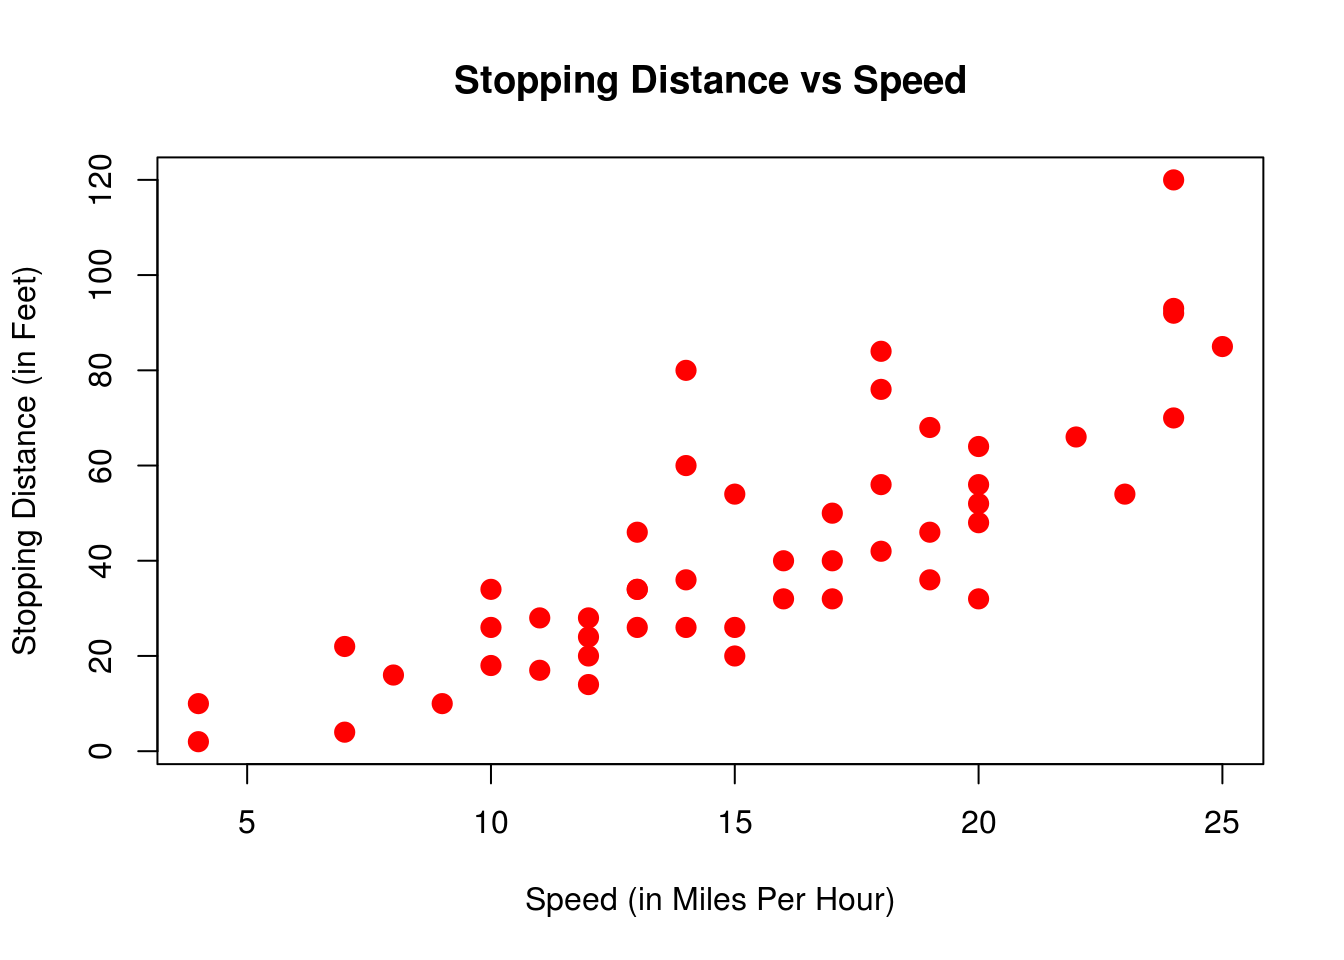
\includegraphics{ScPoEconometrics_files/figure-latex/unnamed-chunk-102-1.pdf}

The histogram function has a number of parameters which can be changed
to make our plot look much nicer. Use the \texttt{?} operator to read
the documentation for the \texttt{hist()} to see a full list of these
parameters.

\begin{Shaded}
\begin{Highlighting}[]
\KeywordTok{hist}\NormalTok{(mpg}\OperatorTok{$}\NormalTok{cty,}
     \DataTypeTok{xlab   =} \StringTok{"Miles Per Gallon (City)"}\NormalTok{,}
     \DataTypeTok{main   =} \StringTok{"Histogram of MPG (City)"}\NormalTok{, }\CommentTok{# main title}
     \DataTypeTok{breaks =} \DecValTok{12}\NormalTok{,   }\CommentTok{# how many breaks?}
     \DataTypeTok{col    =} \StringTok{"red"}\NormalTok{,}
     \DataTypeTok{border =} \StringTok{"blue"}\NormalTok{)}
\end{Highlighting}
\end{Shaded}

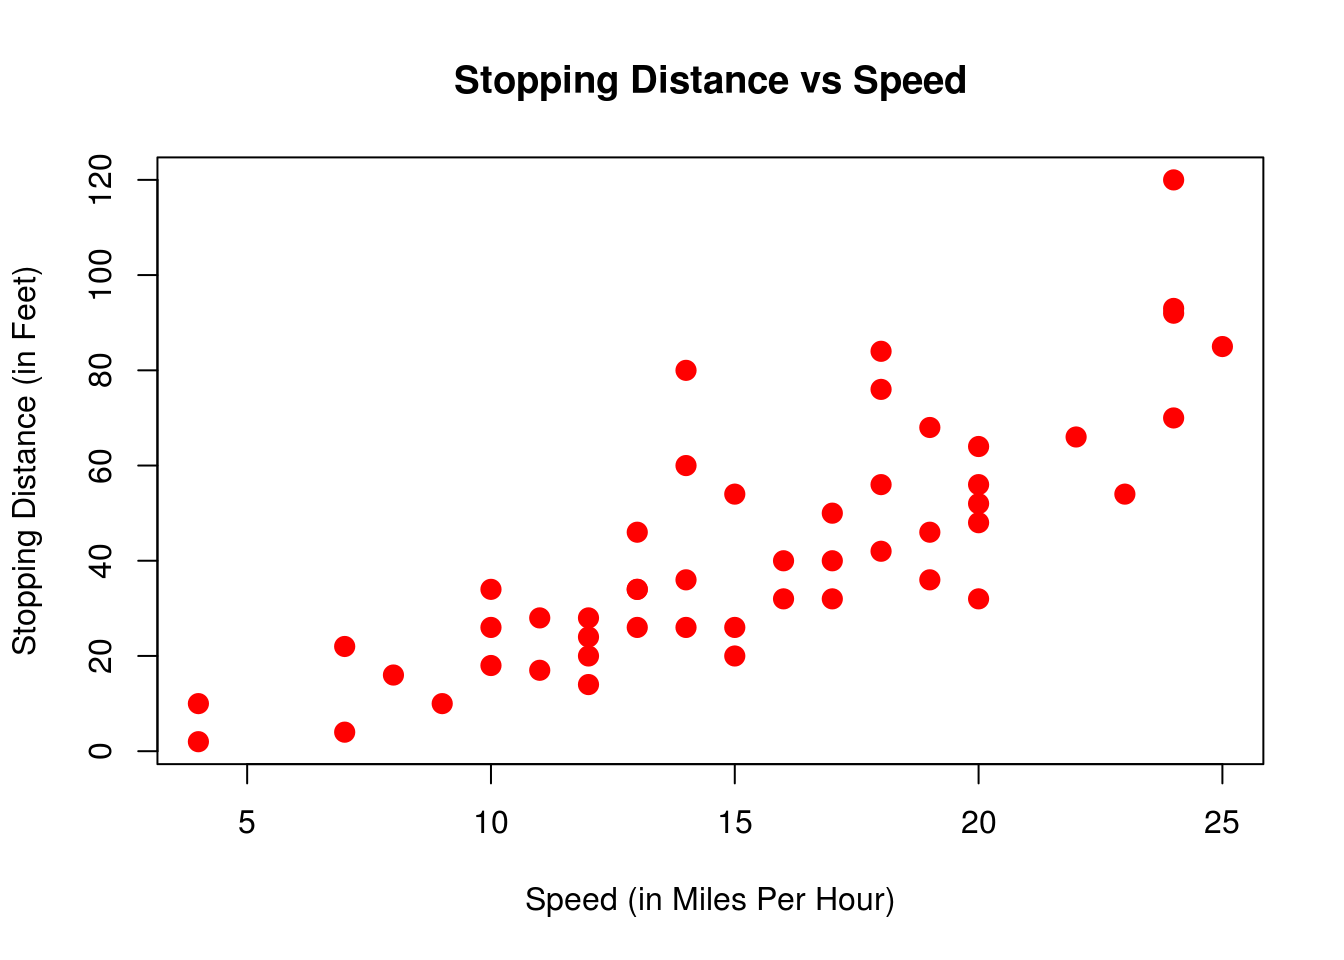
\includegraphics{ScPoEconometrics_files/figure-latex/unnamed-chunk-103-1.pdf}

Importantly, you should always be sure to label your axes and give the
plot a title. The argument \texttt{breaks} is specific to
\texttt{hist()}. Entering an integer will give a suggestion to
\texttt{R} for how many bars to use for the histogram. By default
\texttt{R} will attempt to intelligently guess a good number of
\texttt{breaks}, but as we can see here, it is sometimes useful to
modify this yourself.

\subsection{Barplots}\label{barplots}

Somewhat similar to a histogram, a barplot can provide a visual summary
of a categorical variable, or a numeric variable with a finite number of
values, like a ranking from 1 to 10.

\begin{Shaded}
\begin{Highlighting}[]
\KeywordTok{barplot}\NormalTok{(}\KeywordTok{table}\NormalTok{(mpg}\OperatorTok{$}\NormalTok{drv))}
\end{Highlighting}
\end{Shaded}

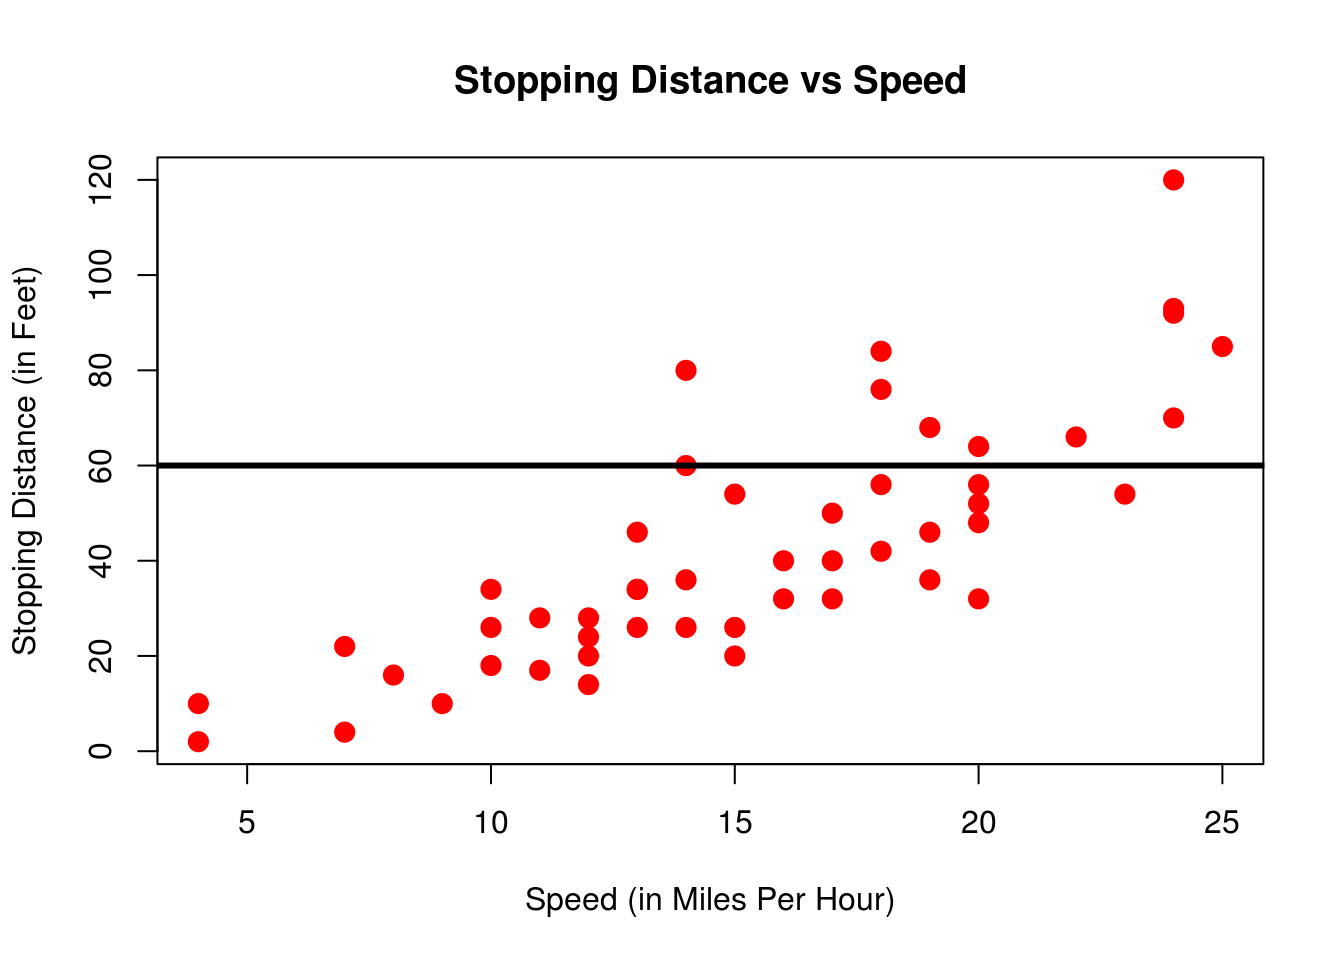
\includegraphics{ScPoEconometrics_files/figure-latex/unnamed-chunk-104-1.pdf}

\begin{Shaded}
\begin{Highlighting}[]
\KeywordTok{barplot}\NormalTok{(}\KeywordTok{table}\NormalTok{(mpg}\OperatorTok{$}\NormalTok{drv),}
        \DataTypeTok{xlab   =} \StringTok{"Drivetrain (f = FWD, r = RWD, 4 = 4WD)"}\NormalTok{,}
        \DataTypeTok{ylab   =} \StringTok{"Frequency"}\NormalTok{,}
        \DataTypeTok{main   =} \StringTok{"Drivetrains"}\NormalTok{,}
        \DataTypeTok{col    =} \StringTok{"dodgerblue"}\NormalTok{,}
        \DataTypeTok{border =} \StringTok{"darkorange"}\NormalTok{)}
\end{Highlighting}
\end{Shaded}

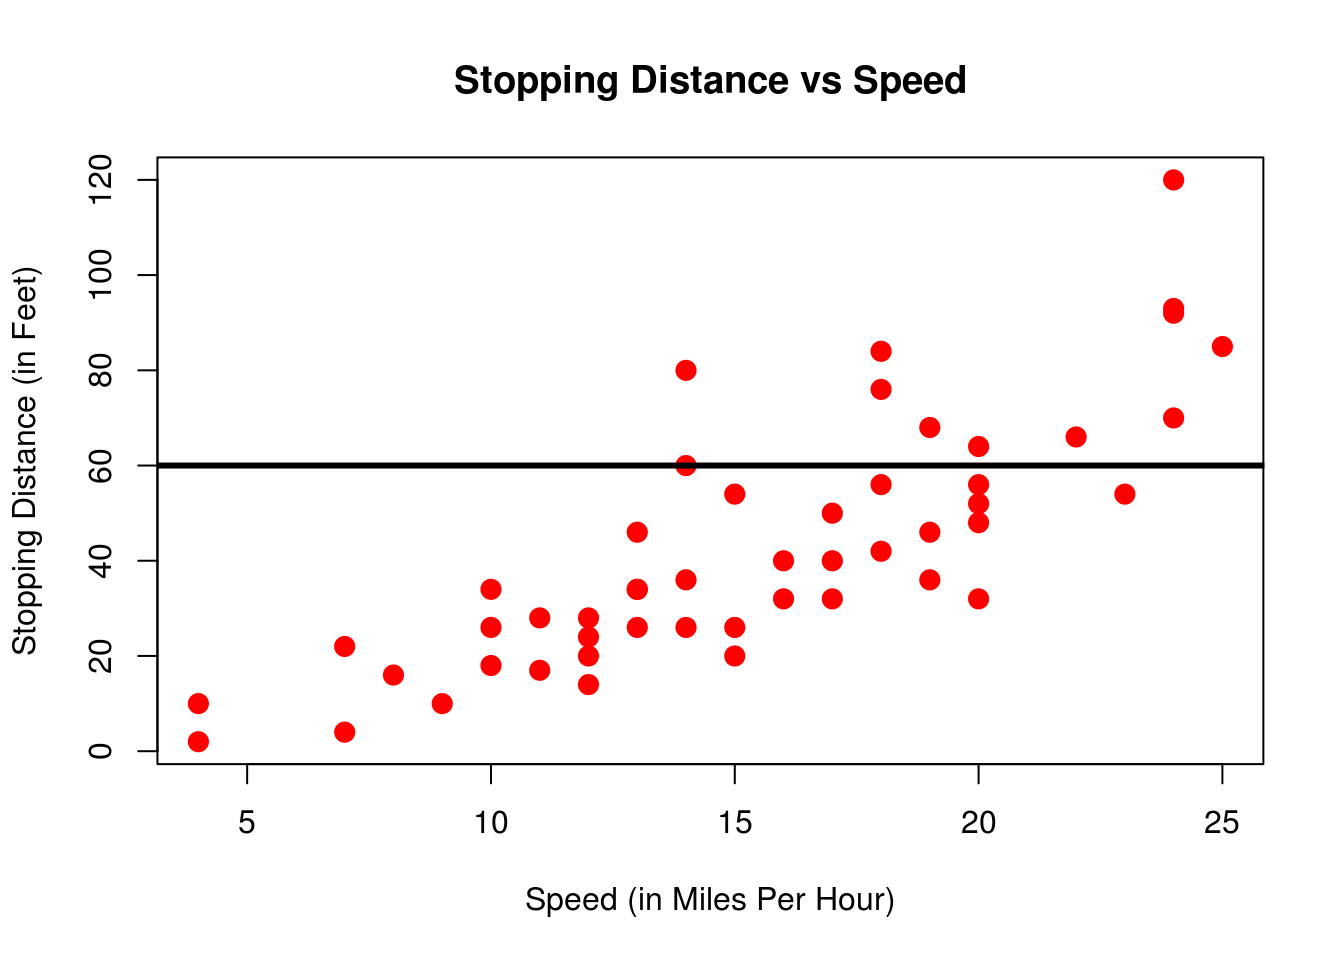
\includegraphics{ScPoEconometrics_files/figure-latex/unnamed-chunk-105-1.pdf}

\subsection{Boxplots}\label{boxplots}

To visualize the relationship between a numerical and categorical
variable, we will use a \textbf{boxplot}. In the \texttt{mpg} dataset,
the \texttt{drv} variable takes a small, finite number of values. A car
can only be front wheel drive, 4 wheel drive, or rear wheel drive.

\begin{Shaded}
\begin{Highlighting}[]
\KeywordTok{unique}\NormalTok{(mpg}\OperatorTok{$}\NormalTok{drv)}
\end{Highlighting}
\end{Shaded}

\begin{verbatim}
## [1] "f" "4" "r"
\end{verbatim}

First note that we can use a single boxplot as an alternative to a
histogram for visualizing a single numerical variable. To do so in
\texttt{R}, we use the \texttt{boxplot()} function.

\begin{Shaded}
\begin{Highlighting}[]
\KeywordTok{boxplot}\NormalTok{(mpg}\OperatorTok{$}\NormalTok{hwy)}
\end{Highlighting}
\end{Shaded}

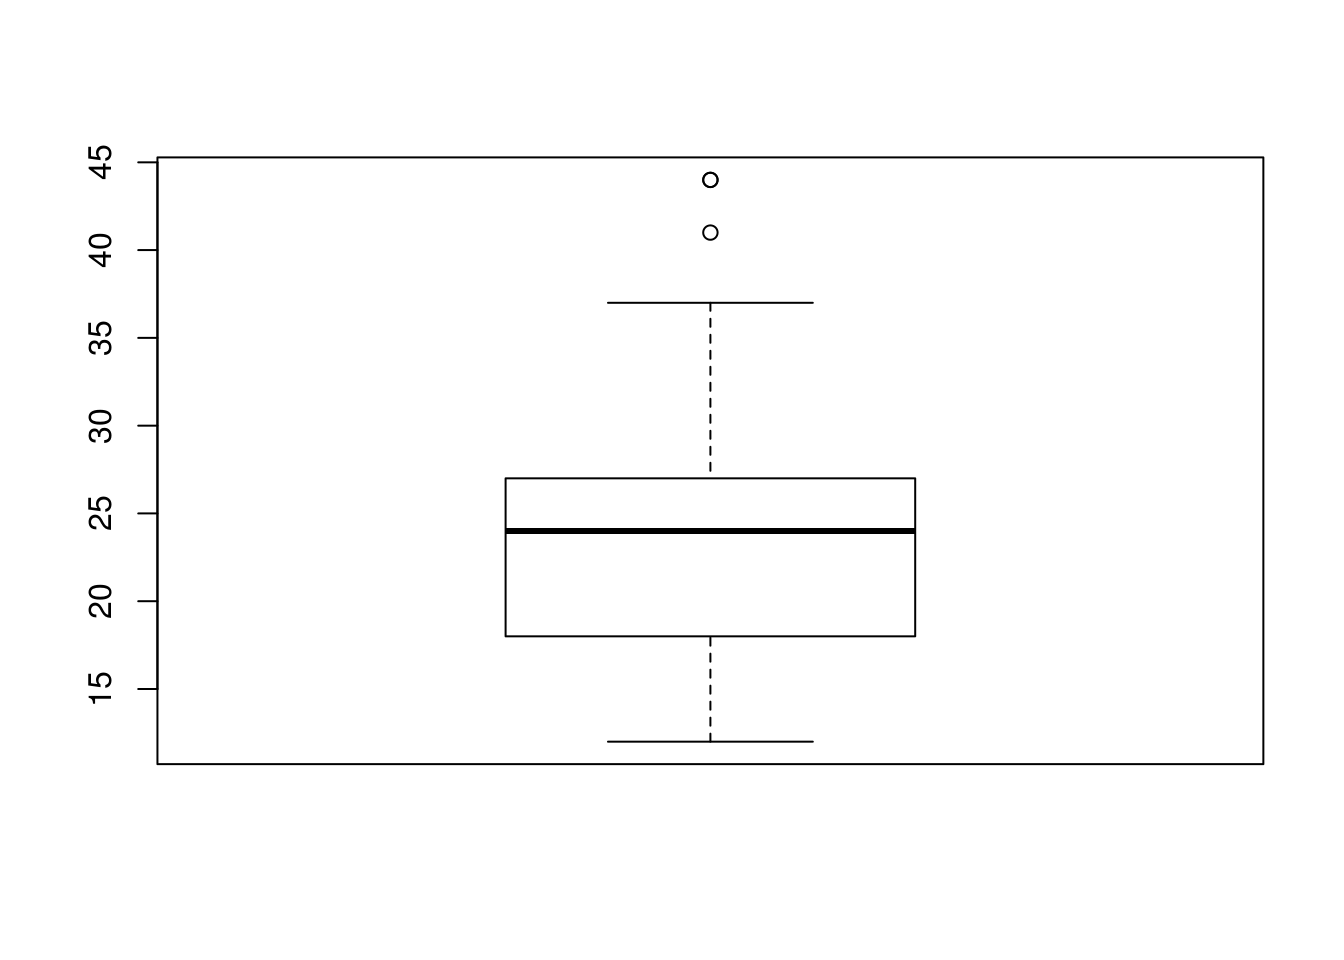
\includegraphics{ScPoEconometrics_files/figure-latex/unnamed-chunk-107-1.pdf}

However, more often we will use boxplots to compare a numerical variable
for different values of a categorical variable.

\begin{Shaded}
\begin{Highlighting}[]
\KeywordTok{boxplot}\NormalTok{(hwy }\OperatorTok{~}\StringTok{ }\NormalTok{drv, }\DataTypeTok{data =}\NormalTok{ mpg)}
\end{Highlighting}
\end{Shaded}

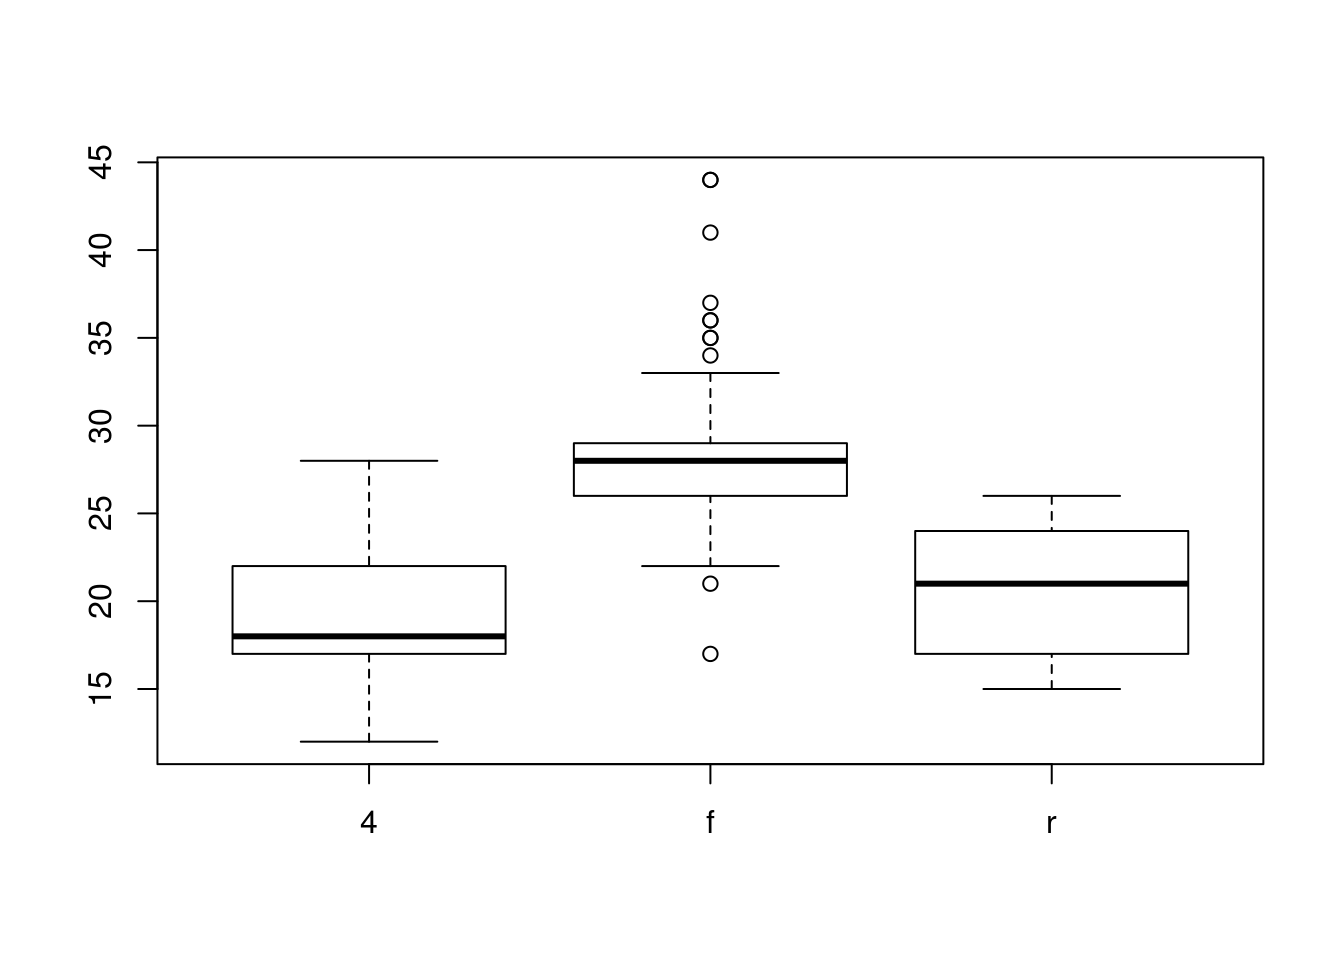
\includegraphics{ScPoEconometrics_files/figure-latex/unnamed-chunk-108-1.pdf}

Here used the \texttt{boxplot()} command to create side-by-side
boxplots. However, since we are now dealing with two variables, the
syntax has changed. The \texttt{R} syntax
\texttt{hwy\ \textasciitilde{}\ drv,\ data\ =\ mpg} reads ``Plot the
\texttt{hwy} variable against the \texttt{drv} variable using the
dataset \texttt{mpg}.'' We see the use of a \texttt{\textasciitilde{}}
(which specifies a formula) and also a \texttt{data\ =} argument. This
will be a syntax that is common to many functions we will use in this
course.

\begin{Shaded}
\begin{Highlighting}[]
\KeywordTok{boxplot}\NormalTok{(hwy }\OperatorTok{~}\StringTok{ }\NormalTok{drv, }\DataTypeTok{data =}\NormalTok{ mpg,}
     \DataTypeTok{xlab   =} \StringTok{"Drivetrain (f = FWD, r = RWD, 4 = 4WD)"}\NormalTok{,}
     \DataTypeTok{ylab   =} \StringTok{"Miles Per Gallon (Highway)"}\NormalTok{,}
     \DataTypeTok{main   =} \StringTok{"MPG (Highway) vs Drivetrain"}\NormalTok{,}
     \DataTypeTok{pch    =} \DecValTok{20}\NormalTok{,}
     \DataTypeTok{cex    =} \DecValTok{2}\NormalTok{,}
     \DataTypeTok{col    =} \StringTok{"darkorange"}\NormalTok{,}
     \DataTypeTok{border =} \StringTok{"dodgerblue"}\NormalTok{)}
\end{Highlighting}
\end{Shaded}

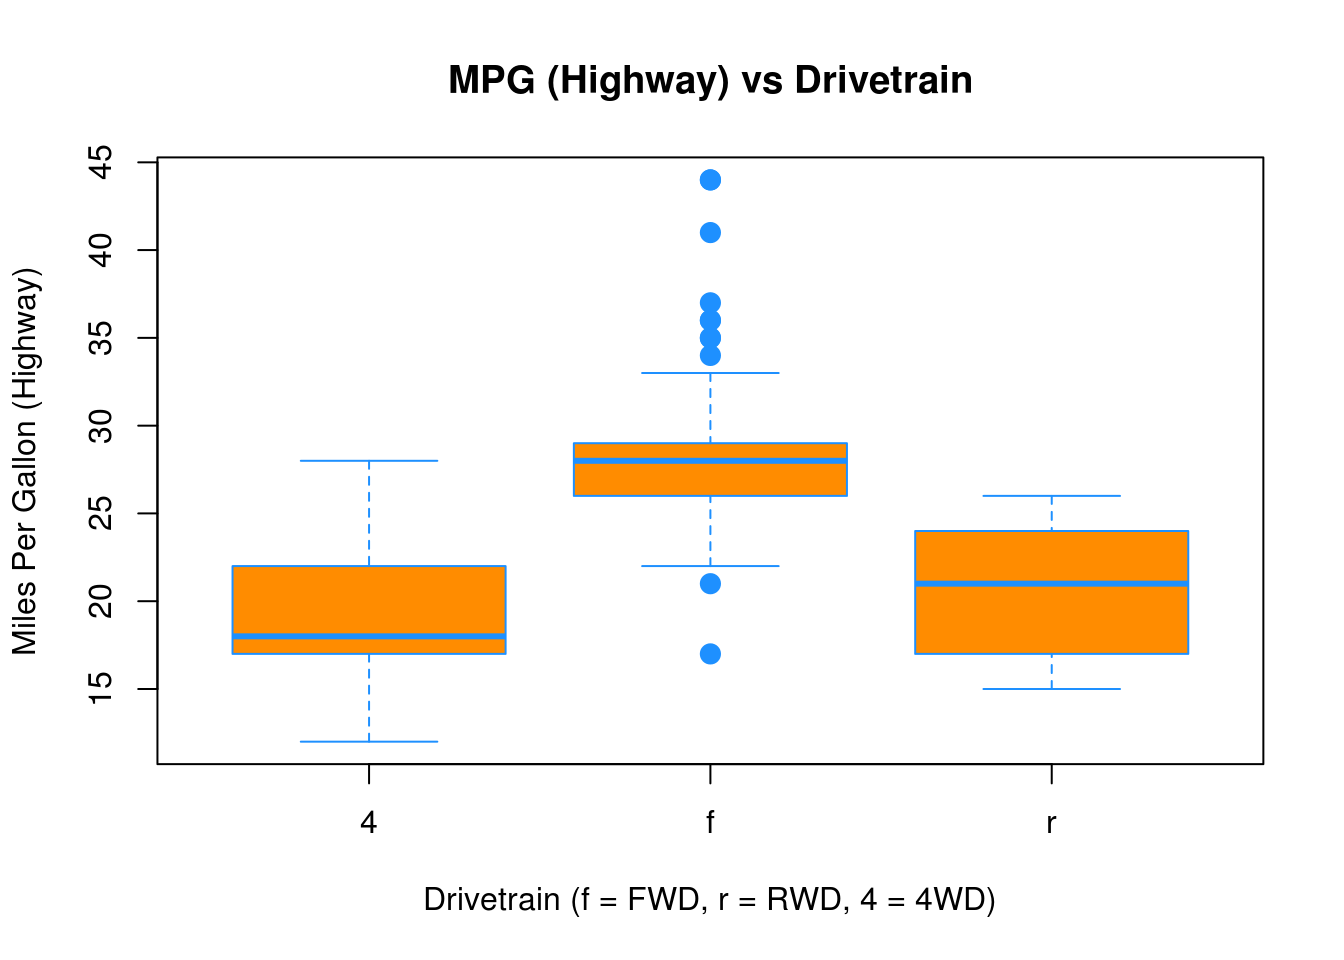
\includegraphics{ScPoEconometrics_files/figure-latex/unnamed-chunk-109-1.pdf}

Again, \texttt{boxplot()} has a number of additional arguments which
have the ability to make our plot more visually appealing.

\subsection{Scatterplots}\label{scatterplots}

Lastly, to visualize the relationship between two numeric variables we
will use a \textbf{scatterplot}. This can be done with the
\texttt{plot()} function and the \texttt{\textasciitilde{}} syntax we
just used with a boxplot. (The function \texttt{plot()} can also be used
more generally; see the documentation for details.)

\begin{Shaded}
\begin{Highlighting}[]
\KeywordTok{plot}\NormalTok{(hwy }\OperatorTok{~}\StringTok{ }\NormalTok{displ, }\DataTypeTok{data =}\NormalTok{ mpg)}
\end{Highlighting}
\end{Shaded}

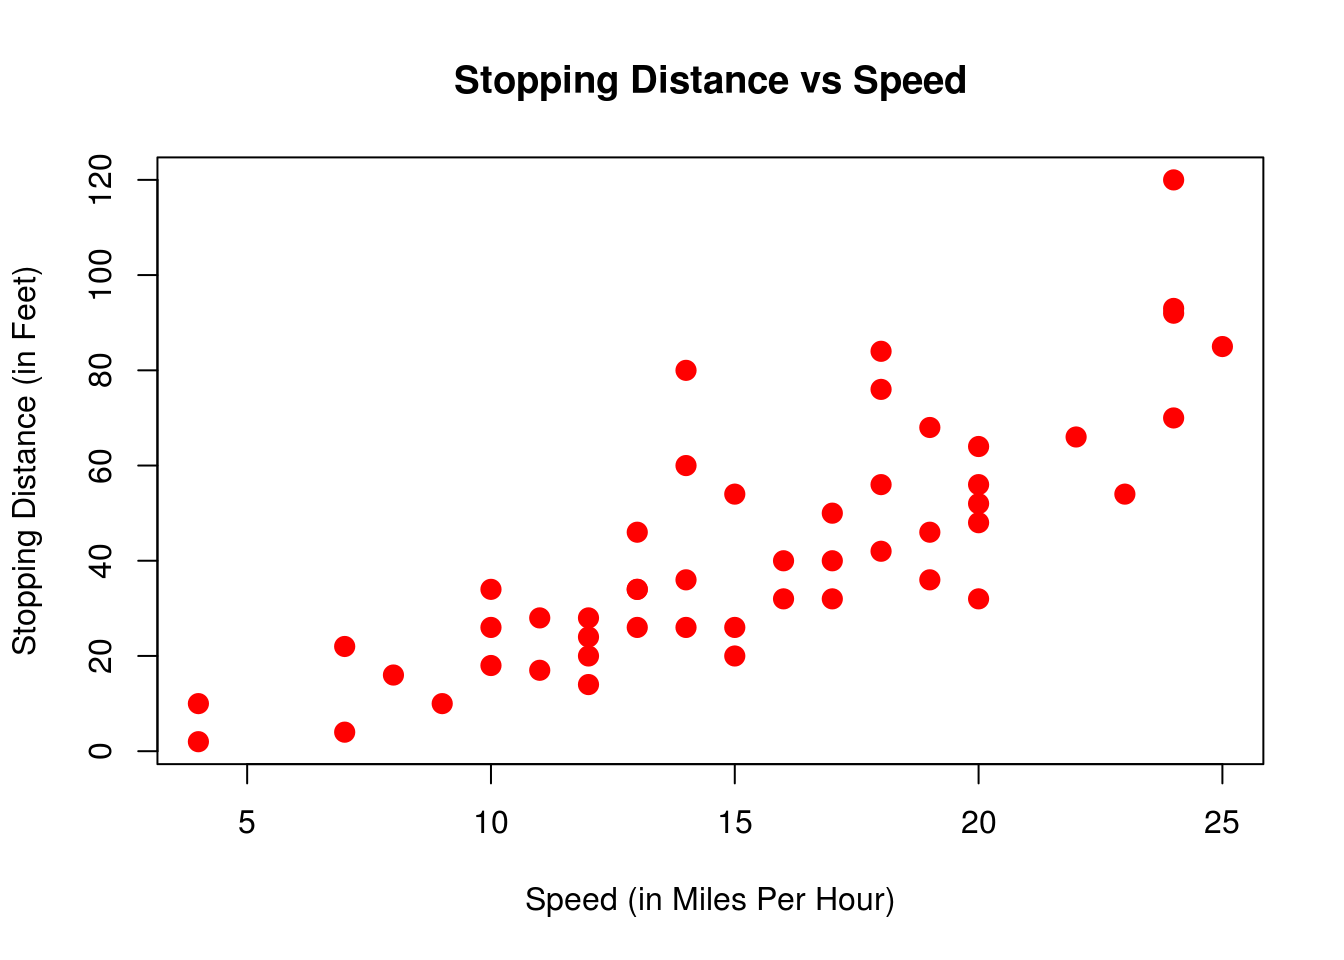
\includegraphics{ScPoEconometrics_files/figure-latex/unnamed-chunk-110-1.pdf}

\begin{Shaded}
\begin{Highlighting}[]
\KeywordTok{plot}\NormalTok{(hwy }\OperatorTok{~}\StringTok{ }\NormalTok{displ, }\DataTypeTok{data =}\NormalTok{ mpg,}
     \DataTypeTok{xlab =} \StringTok{"Engine Displacement (in Liters)"}\NormalTok{,}
     \DataTypeTok{ylab =} \StringTok{"Miles Per Gallon (Highway)"}\NormalTok{,}
     \DataTypeTok{main =} \StringTok{"MPG (Highway) vs Engine Displacement"}\NormalTok{,}
     \DataTypeTok{pch  =} \DecValTok{20}\NormalTok{,}
     \DataTypeTok{cex  =} \DecValTok{2}\NormalTok{,}
     \DataTypeTok{col  =} \StringTok{"dodgerblue"}\NormalTok{)}
\end{Highlighting}
\end{Shaded}

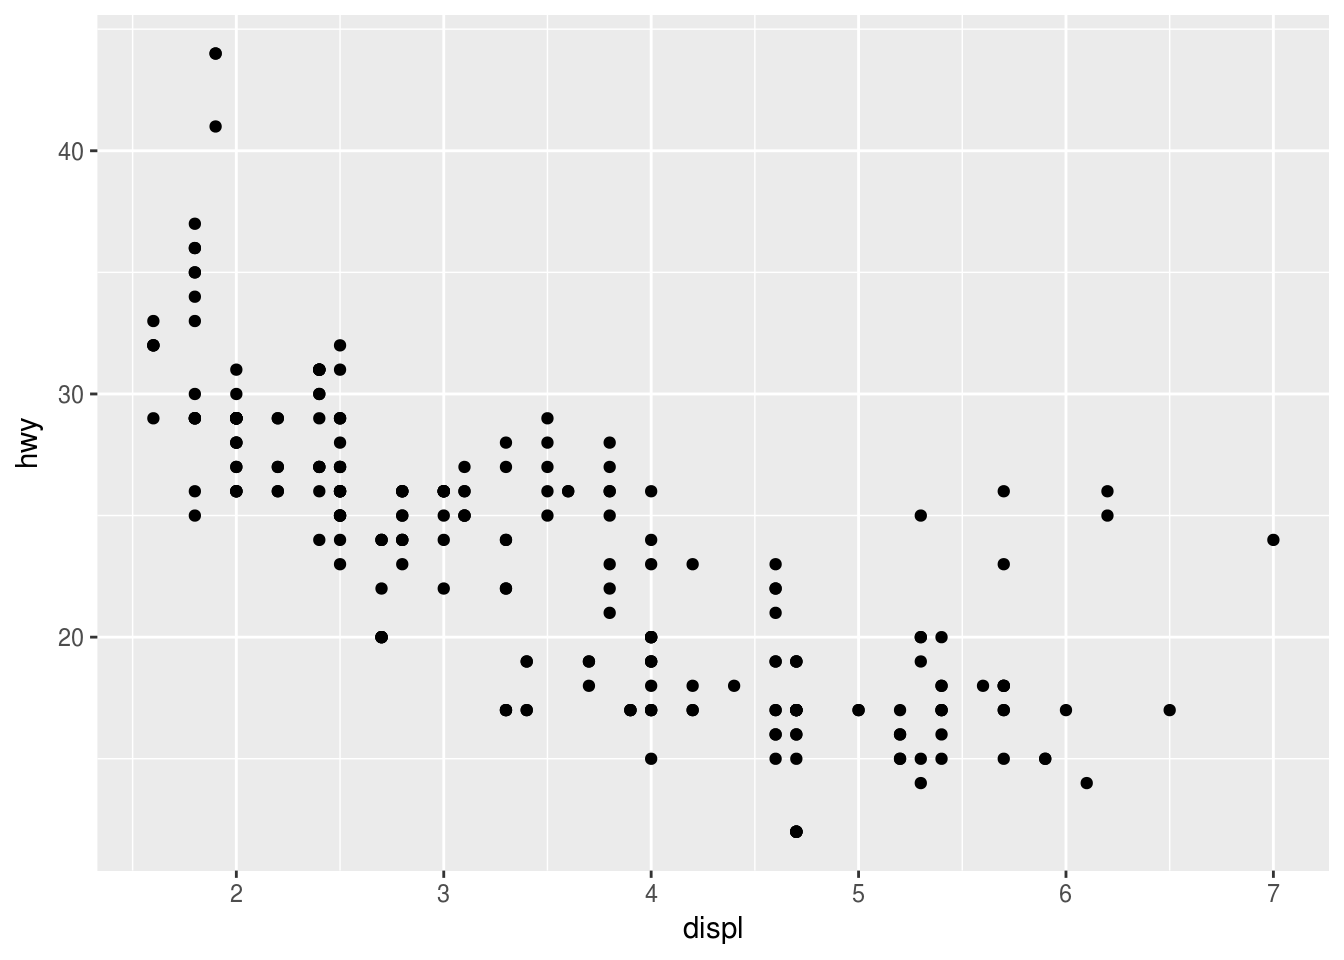
\includegraphics{ScPoEconometrics_files/figure-latex/unnamed-chunk-111-1.pdf}

\subsection{\texorpdfstring{\texttt{ggplot}}{ggplot}}\label{ggplot}

All of the above plots could also have been generate using the
\texttt{ggplot} function from the already loaded \texttt{ggplot2}
package. Which function you use is up to you, but sometimes a plot is
easier to build in base R (like in the \texttt{boxplot} example maybe),
sometimes the other way around.

\begin{Shaded}
\begin{Highlighting}[]
\KeywordTok{ggplot}\NormalTok{(}\DataTypeTok{data =}\NormalTok{ mpg,}\DataTypeTok{mapping =} \KeywordTok{aes}\NormalTok{(}\DataTypeTok{x=}\NormalTok{displ,}\DataTypeTok{y=}\NormalTok{hwy)) }\OperatorTok{+}\StringTok{ }\KeywordTok{geom_point}\NormalTok{()}
\end{Highlighting}
\end{Shaded}

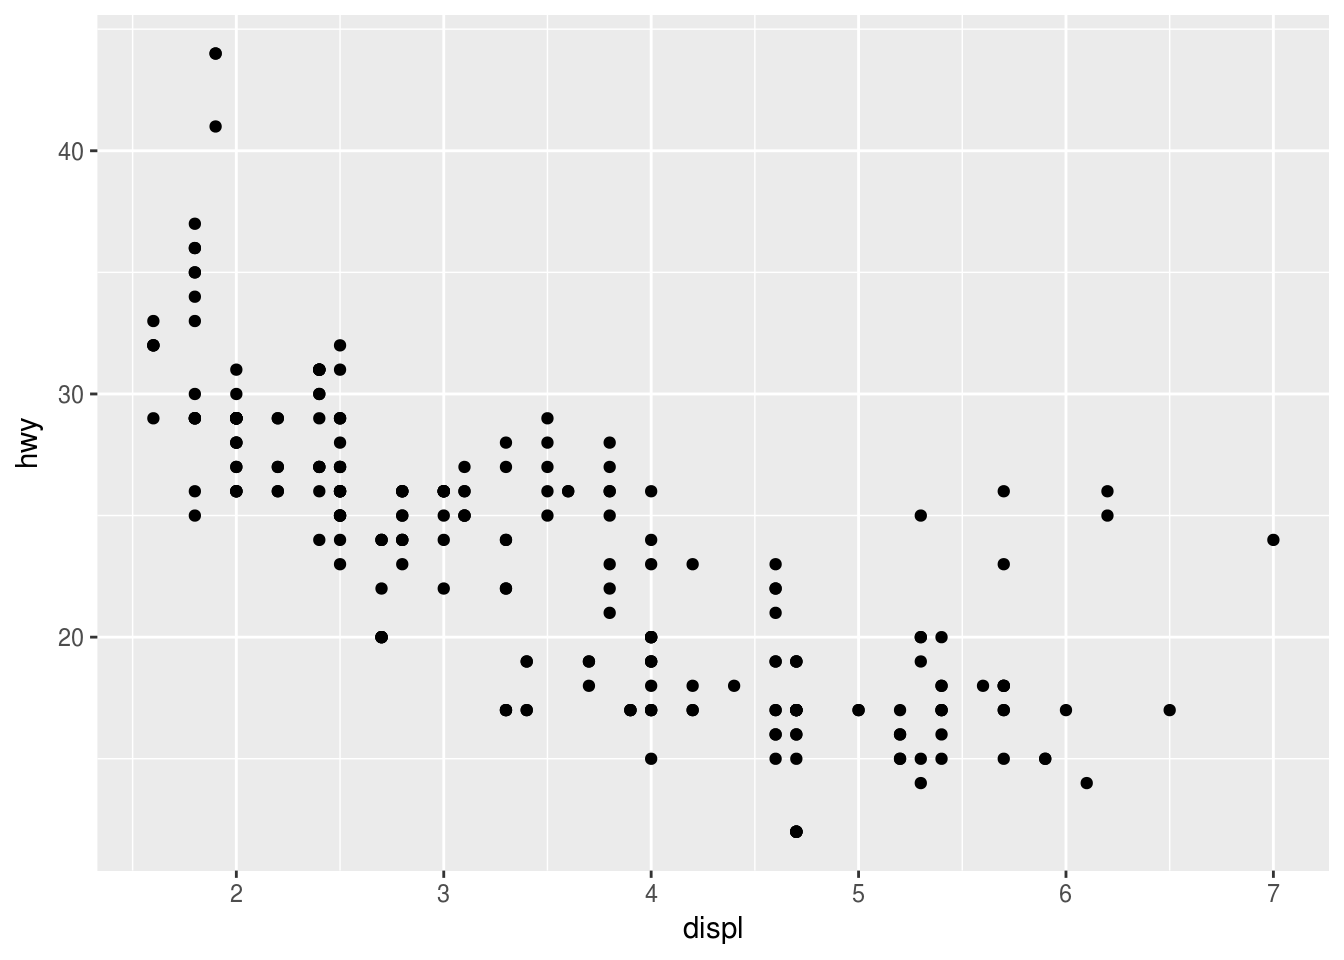
\includegraphics{ScPoEconometrics_files/figure-latex/unnamed-chunk-112-1.pdf}

\texttt{ggplot} is impossible to describe in brief terms, so please look
at \href{http://ggplot2.tidyverse.org}{the package's website} which
provides excellent guidance. We will from time to time use ggplot in
this book, so try to familiarize yourself with it. Let's quickly
demonstrate how one could customize that first plot:

\begin{Shaded}
\begin{Highlighting}[]
\KeywordTok{ggplot}\NormalTok{(}\DataTypeTok{data =}\NormalTok{ mpg, }\DataTypeTok{mapping =} \KeywordTok{aes}\NormalTok{(}\DataTypeTok{x=}\NormalTok{displ,}\DataTypeTok{y=}\NormalTok{hwy)) }\OperatorTok{+}\StringTok{   }\CommentTok{# ggplot() makes base plot}
\StringTok{  }\KeywordTok{geom_point}\NormalTok{(}\DataTypeTok{color=}\StringTok{"blue"}\NormalTok{,}\DataTypeTok{size=}\DecValTok{2}\NormalTok{) }\OperatorTok{+}\StringTok{     }\CommentTok{# how to show x and y?}
\StringTok{  }\KeywordTok{scale_y_continuous}\NormalTok{(}\DataTypeTok{name=}\StringTok{"Miles Per Gallon (Highway)"}\NormalTok{) }\OperatorTok{+}\StringTok{  }\CommentTok{# name of y axis}
\StringTok{  }\KeywordTok{scale_x_continuous}\NormalTok{(}\DataTypeTok{name=}\StringTok{"Engine Displacement (in Liters)"}\NormalTok{) }\OperatorTok{+}\StringTok{ }\CommentTok{# x axis}
\StringTok{  }\KeywordTok{theme_bw}\NormalTok{() }\OperatorTok{+}\StringTok{    }\CommentTok{# change the background}
\StringTok{  }\KeywordTok{ggtitle}\NormalTok{(}\StringTok{"MPG (Highway) vs Engine Displacement"}\NormalTok{)   }\CommentTok{# add a title}
\end{Highlighting}
\end{Shaded}

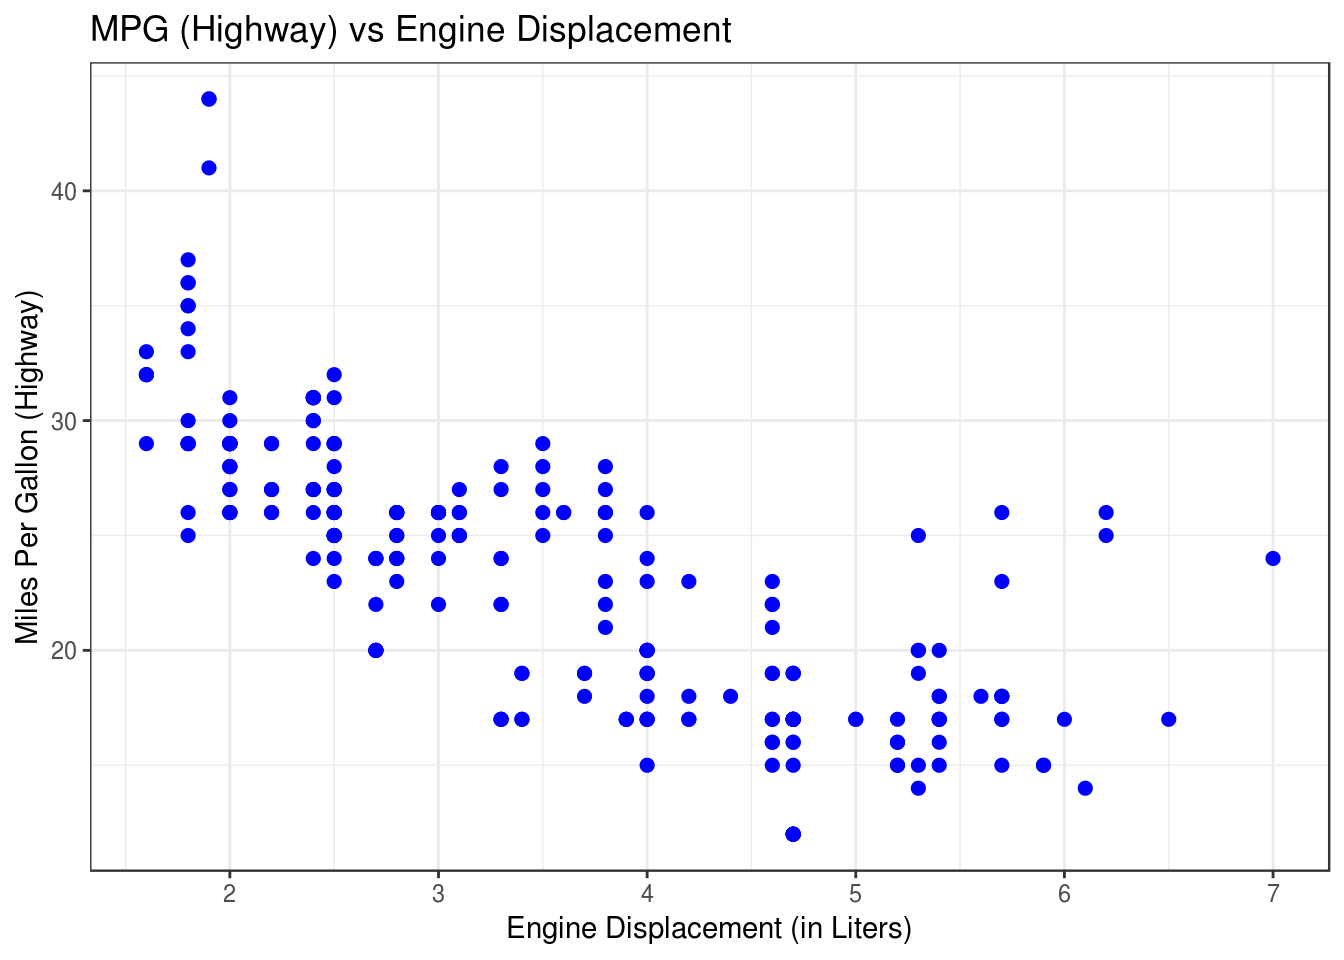
\includegraphics{ScPoEconometrics_files/figure-latex/unnamed-chunk-113-1.pdf}

\section{\texorpdfstring{The
\texttt{tidyverse}}{The tidyverse}}\label{the-tidyverse}

\href{http://hadley.nz}{Hadley Wickham} is the author of R packages
\texttt{ggplot2} and also of \texttt{dplyr} (and also a myriad of
others). With \texttt{ggplot2} he pioneered what he calls the
\emph{grammar of graphics} (hence, \texttt{gg}). Grammar in the sense
that there are \textbf{nouns} and \textbf{verbs} and a \textbf{syntax},
i.e.~rules of how nouns and verbs are to be put together to construct an
understandable sentence. He has extended the \emph{grammar} idea into
various other packages. The \texttt{tidyverse} package is a collection
of those packages.

\texttt{tidy} data is data where:

\begin{itemize}
\tightlist
\item
  Each variable is a column
\item
  Each observation is a row
\item
  Each value is a cell
\end{itemize}

Fair enough, you might say, that is a regular spreadsheet. And you are
right! However, data comes to us \emph{not} tidy most of the times, and
we first need to clean, or \texttt{tidy}, it up. Once it's in
\texttt{tidy} format, we can use the tools in the \texttt{tidyverse}
with great efficiency to analyse the data and stop worrying about which
tool to use.

\subsection{Importing Excel Data}\label{importing-excel-data}

The data we will look at is from
\href{http://ec.europa.eu/eurostat/data/database}{Eurostat} on
demography and migration. You should download the data yourself (click
on previous link, then drill down to \emph{database by themes
\textgreater{} Population and social conditions \textgreater{} Demograph
and migration \textgreater{} Population change - Demographic balance and
crude rates at national level (demo\_gind)}).

Once downloaded, we can read the data with the function
\texttt{read\_excel} from the package
\href{http://readxl.tidyverse.org}{\texttt{readxl}}, again part of the
\texttt{tidyverse} suite.

It's important to know how the data is organized in the spreadsheet.
Open the file with Excel to see:

\begin{itemize}
\tightlist
\item
  There is a heading which we don't need.
\item
  There are 5 rows with info that we don't need.
\item
  There is one table per variable (total population, males, females,
  etc)
\item
  Each table has one row for each country, and one column for each year.
\item
  As such, this data is \textbf{not tidy}.
\end{itemize}

Now we will read the first chunk of data, from the first table:
\emph{total population}:

\begin{Shaded}
\begin{Highlighting}[]
\KeywordTok{library}\NormalTok{(readxl)  }\CommentTok{# load the library}

\CommentTok{# Suppose I downloaded the file to a directory }
\CommentTok{# data/ in my current working directory (cwd)}
\CommentTok{# you can change your cwd with `setwd("your/directory")`}
\CommentTok{# or in RStudio by clicking Session > Set Working Directory}

\CommentTok{# total population in raw format}
\NormalTok{tot_pop_raw =}\StringTok{ }\KeywordTok{read_excel}\NormalTok{(}\DataTypeTok{path =} \StringTok{"data/demo_gind.xls"}\NormalTok{, }
                \DataTypeTok{sheet=}\StringTok{"Data"}\NormalTok{, }\CommentTok{# which sheet}
                \DataTypeTok{range=}\StringTok{"A9:K68"}\NormalTok{)  }\CommentTok{# which excel cell range to read}
\KeywordTok{names}\NormalTok{(tot_pop_raw)[}\DecValTok{1}\NormalTok{] <-}\StringTok{ "Country"}   \CommentTok{# lets rename the first column}
\NormalTok{tot_pop_raw}
\end{Highlighting}
\end{Shaded}

\begin{verbatim}
## # A tibble: 59 x 11
##    Country  `2008` `2009` `2010` `2011` `2012` `2013` `2014` `2015` `2016`
##    <chr>    <chr>  <chr>  <chr>  <chr>  <chr>  <chr>  <chr>  <chr>  <chr> 
##  1 Europea~ 50029~ 50209~ 50317~ 50296~ 50404~ 50516~ 50701~ 50854~ 51027~
##  2 Europea~ 43872~ 44004~ 44066~ 43994~ 44055~ 44125~ 44266~ 44366~ 44489~
##  3 Europea~ 49598~ 49778~ 49886~ 49867~ 49977~ 50090~ 50276~ 50431~ 50608~
##  4 Euro ar~ 33309~ 33447~ 33526~ 33457~ 33528~ 33604~ 33754~ 33856~ 33988~
##  5 Euro ar~ 32988~ 33128~ 33212~ 33152~ 33228~ 33307~ 33459~ 33563~ 33699~
##  6 Belgium  10666~ 10753~ 10839~ 11000~ 11075~ 11137~ 11180~ 11237~ 11311~
##  7 Bulgaria 75180~ 74671~ 74217~ 73694~ 73272~ 72845~ 72456~ 72021~ 71537~
##  8 Czech R~ 10343~ 10425~ 10462~ 10486~ 10505~ 10516~ 10512~ 10538~ 10553~
##  9 Denmark  54757~ 55114~ 55347~ 55606~ 55805~ 56026~ 56272~ 56597~ 57072~
## 10 Germany~ 82217~ 82002~ 81802~ 80222~ 80327~ 80523~ 80767~ 81197~ 82175~
## # ... with 49 more rows, and 1 more variable: `2017` <chr>
\end{verbatim}

This shows a \texttt{tibble}. This is more informative view of a
\texttt{data.frame} (it tells us data type, and how many cols and rows).
Notice, in particular, that \emph{all} columns seem to be of type
\texttt{chr}, i.e.~characters - a string, not a number! We'll have to
fix that, as this is clearly numeric data.

\subsection{\texorpdfstring{\texttt{tidyr}}{tidyr}}\label{tidyr}

In the previous \texttt{tibble}, there is a \emph{hidden} variable:
\texttt{year}. Each year is a column name (like \texttt{2008}) instead
of all years being in one column \texttt{year}. We really would like to
have several rows for each Country, one per year. We want to
\texttt{gather()} all years into a new column to tidy this up - and here
is how:

\begin{enumerate}
\def\labelenumi{\arabic{enumi}.}
\tightlist
\item
  specify which columns are to be gathered: in our case, all years (note
  that \texttt{paste(2008:2017)} produces a vector like
  \texttt{{[}"2008",\ "2009",\ "2010",...{]}})
\item
  say what those columns should be gathered into, i.e.~what is the
  \emph{key} for those values: \texttt{year}.
\item
  Finally, what is the name of the new resulting column, containing the
  \emph{value} from each cell: \texttt{counts}.
\end{enumerate}

\begin{Shaded}
\begin{Highlighting}[]
\KeywordTok{library}\NormalTok{(tidyr)   }\CommentTok{# for the gather function}
\NormalTok{tot_pop =}\StringTok{ }\KeywordTok{gather}\NormalTok{(tot_pop_raw, }\KeywordTok{paste}\NormalTok{(}\DecValTok{2008}\OperatorTok{:}\DecValTok{2017}\NormalTok{),}\DataTypeTok{key=}\StringTok{"year"}\NormalTok{, }\DataTypeTok{value =} \StringTok{"counts"}\NormalTok{)}
\end{Highlighting}
\end{Shaded}

Notice that \texttt{counts} is still a \texttt{chr}. Let's convert it:

\begin{Shaded}
\begin{Highlighting}[]
\NormalTok{tot_pop}\OperatorTok{$}\NormalTok{counts =}\StringTok{ }\KeywordTok{as.integer}\NormalTok{(tot_pop}\OperatorTok{$}\NormalTok{counts)}
\end{Highlighting}
\end{Shaded}

\begin{verbatim}
## Warning: NAs introduced by coercion
\end{verbatim}

\begin{Shaded}
\begin{Highlighting}[]
\NormalTok{tot_pop}
\end{Highlighting}
\end{Shaded}

\begin{verbatim}
## # A tibble: 590 x 3
##    Country                                          year     counts
##    <chr>                                            <chr>     <int>
##  1 European Union (current composition)             2008  500297033
##  2 European Union (without United Kingdom)          2008  438725386
##  3 European Union (before the accession of Croatia) 2008  495985066
##  4 Euro area (19 countries)                         2008  333096775
##  5 Euro area (18 countries)                         2008  329884170
##  6 Belgium                                          2008   10666866
##  7 Bulgaria                                         2008    7518002
##  8 Czech Republic                                   2008   10343422
##  9 Denmark                                          2008    5475791
## 10 Germany (until 1990 former territory of the FRG) 2008   82217837
## # ... with 580 more rows
\end{verbatim}

Now you can see that column \texttt{counts} is indeed a \texttt{int},
i.e.~an integer number, and we are fine.

\subsection{\texorpdfstring{\texttt{dplyr}}{dplyr}}\label{dplyr}

\begin{quote}
The \href{http://r4ds.had.co.nz/transform.html}{transform} chapter of
Hadley Wickham's book is a great place to read up more on using
\texttt{dplyr}.
\end{quote}

With \texttt{dplyr} you can do the following operations on
\texttt{data.frame}s and \texttt{tibble}s:

\begin{itemize}
\tightlist
\item
  Choose observations based on a certain value: \texttt{filter()}
\item
  Reorder rows: \texttt{arrange()}
\item
  Select variables by name: \texttt{select()}
\item
  Create new variables out of existing ones: \texttt{mutate()}
\item
  Summarise variables: \texttt{summarise()}
\end{itemize}

All of those verbs can be used with \texttt{group\_by()}, where we apply
the respective operation on a \emph{group} of the dataframe/tibble. For
example, on our \texttt{tot\_pop} tibble we will now

\begin{itemize}
\tightlist
\item
  filter
\item
  select
\item
  arrange
\end{itemize}

Now we can immediately select some countries and plot their population
over time. We will make use of the \texttt{piping} syntax of
\texttt{dplyr} as already mentioned in section \ref{dataframes}.

\begin{Shaded}
\begin{Highlighting}[]
\KeywordTok{library}\NormalTok{(dplyr)  }\CommentTok{# for %>%, filter, mutate, ...}
\NormalTok{tot_pop }\OperatorTok
\StringTok{  }\KeywordTok{filter}\NormalTok{(Country }\OperatorTok\StringTok{ }\KeywordTok{c}\NormalTok{(}\StringTok{"France"}\NormalTok{,}\StringTok{"United Kingdom"}\NormalTok{,}\StringTok{"Italy"}\NormalTok{,}\StringTok{"Germany"}\NormalTok{)) }\OperatorTok
\StringTok{  }\KeywordTok{mutate}\NormalTok{(}\DataTypeTok{millions =}\NormalTok{ counts }\OperatorTok{/}\StringTok{ }\FloatTok{1e6}\NormalTok{) }\OperatorTok
\StringTok{  }\KeywordTok{ggplot}\NormalTok{(}\DataTypeTok{mapping =} \KeywordTok{aes}\NormalTok{(}\DataTypeTok{x=}\NormalTok{year,}\DataTypeTok{y=}\NormalTok{millions,}\DataTypeTok{color=}\NormalTok{Country,}\DataTypeTok{group=}\NormalTok{Country)) }\OperatorTok{+}\StringTok{ }\KeywordTok{geom_line}\NormalTok{()}
\end{Highlighting}
\end{Shaded}

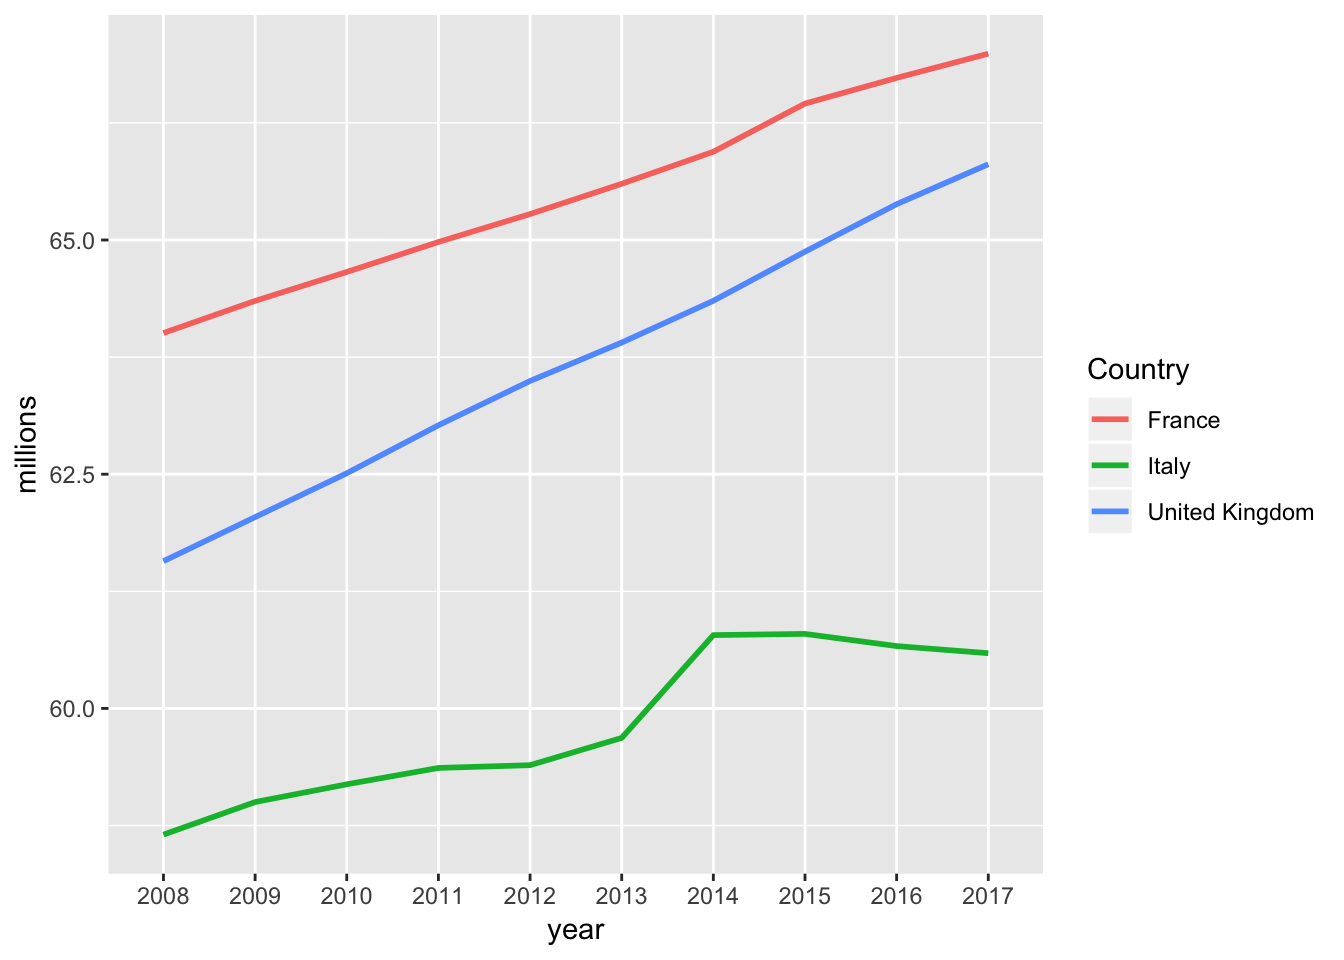
\includegraphics{ScPoEconometrics_files/figure-latex/gather-plot-1.pdf}

\begin{itemize}
\tightlist
\item
  how many NA's?
\item
  plot different vars
\item
  make proportions and plot
\item
  make growth rates and plot
\item
  plot different vars by country
\end{itemize}

\chapter{Linear Regression}\label{linreg}

\begin{enumerate}
\def\labelenumi{\arabic{enumi}.}
\tightlist
\item
  linear regression - stop at R-squared

  \begin{enumerate}
  \def\labelenumii{\arabic{enumii}.}
  \tightlist
  \item
    different data: missing variable
  \item
    non-linear realtionship
  \end{enumerate}
\item
  scatter plot

  \begin{enumerate}
  \def\labelenumii{\arabic{enumii}.}
  \tightlist
  \item
    label observations
  \end{enumerate}
\item
  how do the data come to us? spreadsheet
\item
  approx link x and y by a line
\item
  OLS gives the best line for this

  \begin{enumerate}
  \def\labelenumii{\arabic{enumii}.}
  \tightlist
  \item
    \(y_i = a+b x_i\). find a,b s.t. dist is minimal
  \item
    write out sum of least-squares and call it MSE: u\_1 + u\_2 +
    \ldots{} / N
  \end{enumerate}
\item
  plot fitted values - see imperfect approximation
\item
  R-squared: goodness of fit / measure of goodness

  \begin{enumerate}
  \def\labelenumii{\arabic{enumii}.}
  \tightlist
  \item
    1 - sum of squared errors / SST
  \item
    how much of total variance is explained by the model?
  \end{enumerate}
\item
  regression on mean
\item
  How come there are residuals?

  \begin{enumerate}
  \def\labelenumii{\arabic{enumii}.}
  \tightlist
  \item
    measurement error?
  \item
    there is more to this than just x
  \item
    misspecification
  \end{enumerate}
\item
  There is statistical uncertainty about those estimates
\item
  plot a second data set with a less clear interpretation

  \begin{enumerate}
  \def\labelenumii{\arabic{enumii}.}
  \tightlist
  \item
    do you \emph{really} think there is a linear relationship?
  \item
    SE tells us whethe rwe really think this is a positive slope
  \item
    poor R2 and large standard error
  \item
    How \textbf{confident} are you about this relationship? Is there
    enought data?
  \item
    SE is ameasure of precision depending on N
  \end{enumerate}
\end{enumerate}

\section{Try to find the Slope!}\label{try-to-find-the-slope}

\begin{Shaded}
\begin{Highlighting}[]
\NormalTok{knitr}\OperatorTok{::}\KeywordTok{include_url}\NormalTok{(}\StringTok{"https://gallery.shinyapps.io/simple_regression/"}\NormalTok{)}
\end{Highlighting}
\end{Shaded}

\chapter{Standard Errors}\label{std-errors}

\begin{enumerate}
\def\labelenumi{\arabic{enumi}.}
\tightlist
\item
  Standard Errors

  \begin{enumerate}
  \def\labelenumii{\arabic{enumii}.}
  \tightlist
  \item
    True data
  \item
    play with N and see how errors behave
  \end{enumerate}
\end{enumerate}

\chapter{Multiple Regression}\label{multiple-reg}

\begin{itemize}
\tightlist
\item
  Same as simple regression but more variables
\item
  income \textasciitilde{} age is not linear
\end{itemize}

\begin{Shaded}
\begin{Highlighting}[]
\NormalTok{knitr}\OperatorTok{::}\KeywordTok{include_app}\NormalTok{(}\StringTok{"https://gallery.shinyapps.io/multi_regression/"}\NormalTok{,}\DataTypeTok{height=}\StringTok{"1600px"}\NormalTok{)}
\end{Highlighting}
\end{Shaded}

\chapter{Categorial Variables: Dummies and
Interactions}\label{categorical-vars}

\begin{enumerate}
\def\labelenumi{\arabic{enumi}.}
\tightlist
\item
  if you only have educ categories, the estimate is like the conditional
  mean by educ
\item
  if you have too many categories you will have empty bins
\end{enumerate}

\chapter{Quantile Regression}\label{quantreg}

\begin{enumerate}
\def\labelenumi{\arabic{enumi}.}
\tightlist
\item
  before you were modelling the mean. the average link
\item
  now what happens to \textbf{outliers}? how robust is the mean to that
\item
  what about the entire distribution of this?
\end{enumerate}

\chapter{Panel Data}\label{panel-data}

\begin{itemize}
\tightlist
\item
  scanner data on breakfast cereals, \((Q_{it},D_{it})\)
\item
  why does D vary with Q
\item
  pos relation ship
\item
  don't observe the group identity!
\item
  unobserved het alpha is correlated with Q
\item
  within group estimator
\item
  what if you don't have panel data?
\end{itemize}

\chapter{Instrumental Variables}\label{IV}

\begin{enumerate}
\def\labelenumi{\arabic{enumi}.}
\tightlist
\item
  wage = educ
\item
  educ = ability
\item
  ols estimator captures your ability
\item
  you predict x by z and you only keep the variation that is in the
  error
\end{enumerate}

\chapter{Logit and Probit}\label{logit-probit}

\chapter{Principal Component Analysis}\label{pca}

\chapter{Notes}\label{notes}

this creates a library for the used R packages.

In order to install that package, you need to do

\begin{Shaded}
\begin{Highlighting}[]
\ControlFlowTok{if}\NormalTok{ (}\OperatorTok{!}\KeywordTok{require}\NormalTok{(devtools))\{}
  \KeywordTok{install.packages}\NormalTok{(}\StringTok{"devtools"}\NormalTok{)}
\NormalTok{\}}
\KeywordTok{library}\NormalTok{(devtools)}
\KeywordTok{install_github}\NormalTok{(}\StringTok{"floswald/ScPoEconometrics"}\NormalTok{)  }
\end{Highlighting}
\end{Shaded}

\section{Book usage}\label{book-usage}

You can label chapter and section titles using \texttt{\{\#label\}}
after them, e.g., we can reference Chapter \ref{intro}. If you do not
manually label them, there will be automatic labels anyway, e.g.,
Chapter \ref{linreg}.

Figures and tables with captions will be placed in \texttt{figure} and
\texttt{table} environments, respectively.

\begin{Shaded}
\begin{Highlighting}[]
\KeywordTok{par}\NormalTok{(}\DataTypeTok{mar =} \KeywordTok{c}\NormalTok{(}\DecValTok{4}\NormalTok{, }\DecValTok{4}\NormalTok{, .}\DecValTok{1}\NormalTok{, .}\DecValTok{1}\NormalTok{))}
\KeywordTok{plot}\NormalTok{(pressure, }\DataTypeTok{type =} \StringTok{'b'}\NormalTok{, }\DataTypeTok{pch =} \DecValTok{19}\NormalTok{)}
\end{Highlighting}
\end{Shaded}

\begin{figure}

{\centering 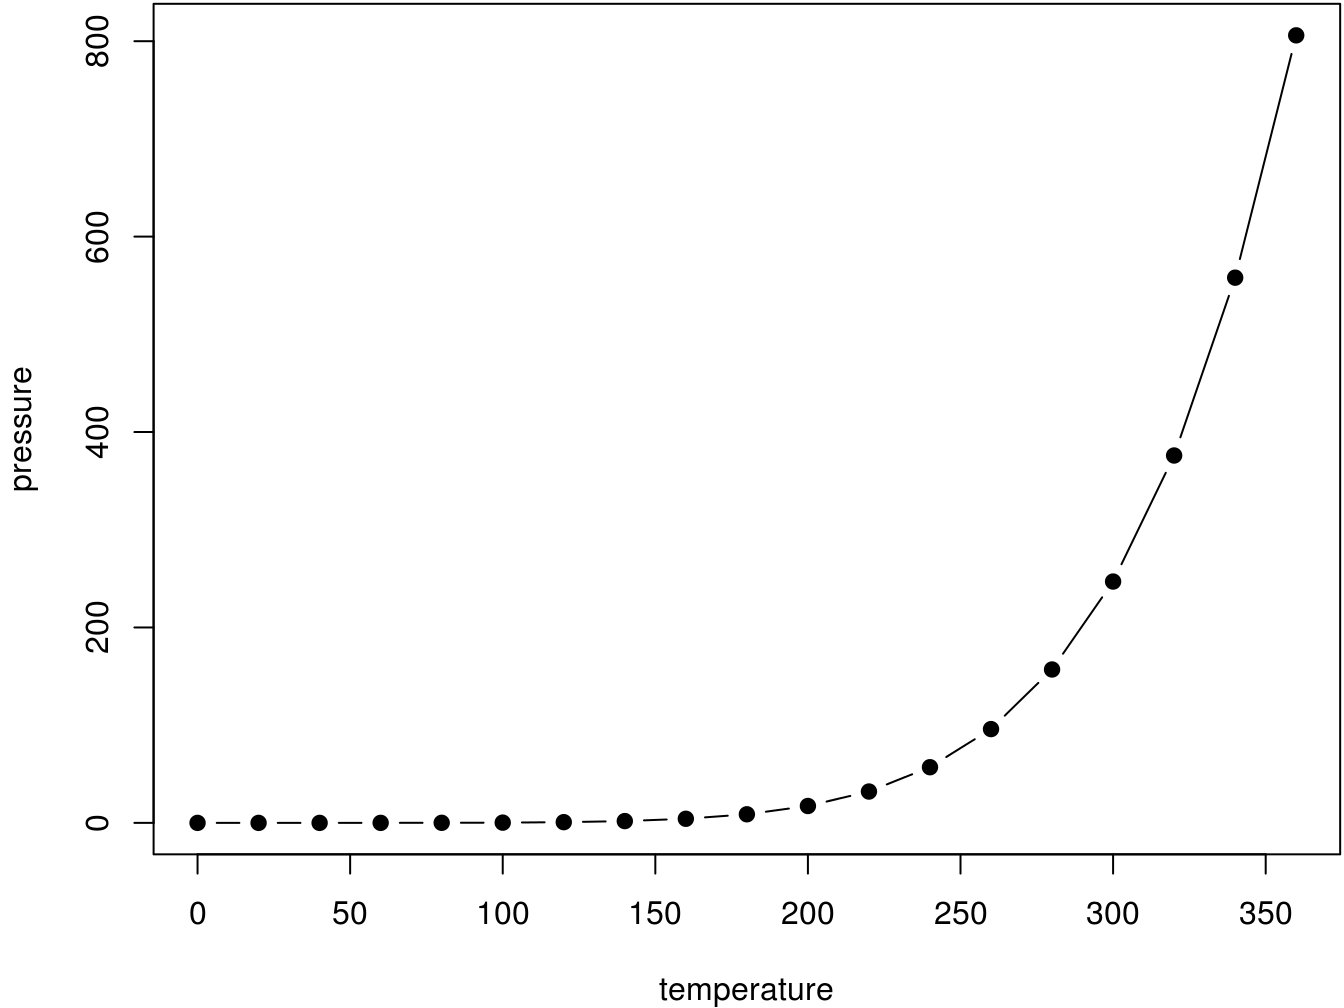
\includegraphics[width=0.8\linewidth]{ScPoEconometrics_files/figure-latex/nice-fig-1} 

}

\caption{Here is a nice figure!}\label{fig:nice-fig}
\end{figure}

Reference a figure by its code chunk label with the \texttt{fig:}
prefix, e.g., see Figure \ref{fig:nice-fig}. Similarly, you can
reference tables generated from \texttt{knitr::kable()}, e.g., see Table
\ref{tab:nice-tab}.

\begin{Shaded}
\begin{Highlighting}[]
\NormalTok{knitr}\OperatorTok{::}\KeywordTok{kable}\NormalTok{(}
  \KeywordTok{head}\NormalTok{(iris, }\DecValTok{20}\NormalTok{), }\DataTypeTok{caption =} \StringTok{'Here is a nice table!'}\NormalTok{,}
  \DataTypeTok{booktabs =} \OtherTok{TRUE}
\NormalTok{)}
\end{Highlighting}
\end{Shaded}

\begin{table}

\caption{\label{tab:nice-tab}Here is a nice table!}
\centering
\begin{tabular}[t]{rrrrl}
\toprule
Sepal.Length & Sepal.Width & Petal.Length & Petal.Width & Species\\
\midrule
5.1 & 3.5 & 1.4 & 0.2 & setosa\\
4.9 & 3.0 & 1.4 & 0.2 & setosa\\
4.7 & 3.2 & 1.3 & 0.2 & setosa\\
4.6 & 3.1 & 1.5 & 0.2 & setosa\\
5.0 & 3.6 & 1.4 & 0.2 & setosa\\
\addlinespace
5.4 & 3.9 & 1.7 & 0.4 & setosa\\
4.6 & 3.4 & 1.4 & 0.3 & setosa\\
5.0 & 3.4 & 1.5 & 0.2 & setosa\\
4.4 & 2.9 & 1.4 & 0.2 & setosa\\
4.9 & 3.1 & 1.5 & 0.1 & setosa\\
\addlinespace
5.4 & 3.7 & 1.5 & 0.2 & setosa\\
4.8 & 3.4 & 1.6 & 0.2 & setosa\\
4.8 & 3.0 & 1.4 & 0.1 & setosa\\
4.3 & 3.0 & 1.1 & 0.1 & setosa\\
5.8 & 4.0 & 1.2 & 0.2 & setosa\\
\addlinespace
5.7 & 4.4 & 1.5 & 0.4 & setosa\\
5.4 & 3.9 & 1.3 & 0.4 & setosa\\
5.1 & 3.5 & 1.4 & 0.3 & setosa\\
5.7 & 3.8 & 1.7 & 0.3 & setosa\\
5.1 & 3.8 & 1.5 & 0.3 & setosa\\
\bottomrule
\end{tabular}
\end{table}

You can write citations, too. For example, we are using the
\textbf{bookdown} package \citep{R-bookdown} in this sample book, which
was built on top of R Markdown and \textbf{knitr} \citep{xie2015}.

\bibliography{book.bib,packages.bib}


\end{document}
